%====================================================
% DAVIS — Academic Draft (v0.1)
%====================================================
\documentclass[11pt]{article}
\usepackage{amsmath}
% ---------- Encoding & Fonts ----------
\usepackage[T1]{fontenc}
\usepackage[utf8]{inputenc}
\usepackage{microtype}
\usepackage{lmodern}
\usepackage{newunicodechar}
\usepackage{pifont}
\usepackage{pgfplots}
\newunicodechar{→}{\textrightarrow{}}
\newunicodechar{∼}{\textasciitilde{}}
\newunicodechar{≤}{\ensuremath{\leq}}
\newunicodechar{−}{\ensuremath{-}}
\newunicodechar{≈}{\ensuremath{\approx}}

% ---------- Page Layout ----------
\usepackage[margin=1in]{geometry}
\usepackage{setspace}
\setstretch{1.08}

% ---------- Math & Symbols ----------
\usepackage{amsmath,amssymb,amsfonts,amsthm,bm}
\usepackage{mathtools}
\usepackage{tabularx}
\usepackage{siunitx}
\sisetup{detect-all=true}
\DeclareMathOperator*{\argmin}{arg\,min}
\DeclareMathOperator*{\argmax}{arg\,max}
\newcommand{\E}{\mathbb{E}}
\newcommand{\Prob}{\mathbb{P}}
\newcommand{\Var}{\mathrm{Var}}
\newcommand{\norm}[1]{\left\lVert #1 \right\rVert}
\newcommand{\RR}{\mathbb{R}}

% ---------- Graphics & Tables ----------
\usepackage{graphicx}
\usepackage{booktabs}
\usepackage{multirow}
\usepackage{adjustbox}

% ---------- Framed Boxes (for novelty framing, checklists) ----------
\usepackage{mdframed}
\usepackage{xcolor}

% ---------- Algorithms ----------
\usepackage{algorithm}
\usepackage{algpseudocode}
\usepackage{float}  % Critical for [H] placement

% Prevent algorithms from floating away
\makeatletter
\renewcommand{\fps@algorithm}{htbp}
\setcounter{totalnumber}{10}
\setcounter{topnumber}{10}
\setcounter{bottomnumber}{10}
\renewcommand{\topfraction}{0.9}
\renewcommand{\bottomfraction}{0.9}
\renewcommand{\textfraction}{0.1}
\renewcommand{\floatpagefraction}{0.8}
\makeatother
\setlength{\intextsep}{10pt plus 2pt minus 2pt}

% ---------- Links & Clever Refs ----------
\usepackage[hidelinks]{hyperref}
\usepackage[capitalise,nameinlink]{cleveref}

% ---------- Quotes & Lists ----------
\usepackage{csquotes}
\usepackage{enumitem}
\setlist[itemize]{leftmargin=*, itemsep=2pt, topsep=2pt}
\setlist[enumerate]{leftmargin=*, itemsep=2pt, topsep=2pt}

% ---------- Theorem Envs ----------
\newtheorem{definition}{Definition}
\newtheorem{theorem}{Theorem}
\newtheorem{lemma}{Lemma}
\newtheorem{proposition}{Proposition}
\newtheorem{corollary}{Corollary}

% ---------- Title Block ----------
\title{\textbf{The Davis Manifold}\\[0.5ex]
\large Geometry-First Detection with Compositional Error Budgets}
\author{Bee Rosa Davis\\
\small NASA Mission Systems Engineer\\
\small \texttt{bee\_davis@alumni.brown.edu}}
\date{} % (leave empty for no date)

% Optional: TOC polish
\usepackage{tocloft}

\begin{document}
\maketitle
\vspace{-1.5ex}

\begin{abstract}
Many safety-critical detection problems have a common structure: an underlying configuration
(e.g., antigenic profile, real human identity, physical pose) evolves along identity-preserving
paths, while only indirect, noisy observations are available. Contemporary machine-learning
systems typically treat these problems as static classification or black-box sequence modeling,
conflating Euclidean similarity in a learned embedding with semantic stability, and providing
few explicit regimes of validity, abstention rules, or decomposed error budgets.

We introduce \emph{Davis manifolds} and \emph{Davis systems} as a general framework for
geometry-first detection in identity-preserving temporal domains. A Davis manifold is a
Riemannian state space equipped with (i) path classes $\mathcal{P}(L)$ describing ``benign''
identity-preserving trajectories of bounded length $L$, (ii) a bounded geodesic--Euclidean
distortion profile $\varepsilon(L)$ along these paths, and (iii) soft/hard configuration margins
$(\kappa_{\mathrm{hard}}, \kappa_{\mathrm{soft}})$ that carve out an explicit ambiguity band where the
system must abstain. A Davis system couples such a manifold to (iv) monotone
path-based features and a scalar statistic $S$, (v) a finite-variance tail bound (Cantelli
inequality) mapping separation in $S$ to misclassification risk, and (vi) a compositional
error budget over geometry, feature linkage, calibration, and abstention failures.

Formally, we (1) define Davis manifolds and Davis systems and state core assumptions
(A1--A6) together with non-vacuity conditions that ensure configuration margins are not
destroyed by distortion; (2) prove an existence theorem showing that contrastive training
(InfoNCE) plus smoothness regularization yields Davis manifolds with explicit
$\varepsilon(L) \leq K(\lambda)L$ dependence on regularization strength and path horizon;
(3) derive finite-variance detection bounds in which posterior correctness decomposes into
a Cantelli term and a multiplicative error budget $(1-E_{\text{geom}})(1-E_{\text{link}})
(1-\xi)(1-\zeta)$ corrected by an independence slack $\delta_{\text{indep}}$; (4) analyze the
trade-off between path length $L$ and distortion $\varepsilon(L)$ and describe how to choose
an operational horizon $L_\star$ that balances coverage against geometric stability; and
(5) instantiate the framework in two domains---HERALD for viral antigenic drift and
VIDAR for deepfake detection via identity trajectories---as worked Davis systems.

\emph{Scope}: This manuscript is conceptual. It states definitions, assumptions, theorems,
and proposed empirical protocols (including distortion audits, error-budget estimation,
and abstention monitoring) but does not report retrospective or prospective performance
metrics. Within this scope, Davis manifolds provide a unifying geometric foundation for
identity-preserving temporal detection with explicit regimes of validity, abstention as a
first-class behavior, and compositional error budgets that make failures legible and
falsifiable.
\end{abstract}

\section{Introduction}
\label{sec:intro}

Many high-stakes learning problems involve \emph{identity-preserving temporal processes}: viruses drifting through antigenic space while remaining the ``same'' lineage; faces moving through pose and illumination while remaining the same person; robots traversing a workspace while preserving object identity. In all of these cases, what matters is not just what an observation \emph{looks like} in isolation, but how it \emph{moves} in a latent space where distance has semantic meaning.

Standard pipelines blur three distinct questions:
\begin{enumerate}[leftmargin=*]
    \item \textbf{Construction}: How do we construct a representation in which distances and paths correspond to meaningful functional changes?
    \item \textbf{Traversal}: Given such a representation, how do we monitor trajectories and build detection statistics?
    \item \textbf{Guarantees}: Under what \emph{explicit} assumptions can we bound risk, expose failure modes, and abstain when the regime of validity is violated?
\end{enumerate}
Most deep learning work optimizes traversal---architectures and losses---on top of whatever representation emerges, and then reports empirical metrics. Geometry, if present, is implicit and un-audited; uncertainty, abstention, and error budgets are usually bolted on post hoc.

\paragraph{Key idea.}
We propose to reverse this order. A \emph{Davis manifold} is a learned (or inherited) Riemannian manifold on which:
\begin{itemize}[leftmargin=*]
    \item geodesic distance $d_g$ is constructed to reflect semantic change along identity-preserving paths;
    \item Euclidean computations in an ambient embedding are guaranteed to approximate $d_g$ within a \emph{bounded-distortion regime} parameterized by $\varepsilon(L)$, the distortion radius for paths of length at most $L$;
    \item configuration regions (``similar'', ``changed'', ``ambiguous'') are separated by soft/hard margins $(\kappa_{\text{hard}}, \kappa_{\text{soft}})$, with ambiguity explicitly mapped to abstention;
    \item downstream detection statistics admit finite-variance risk bounds with decomposed error budgets---geometry, linkage, calibration, and abstention each have their own terms.
\end{itemize}
A \emph{Davis system} couples such a manifold with path families, features, aggregation, and abstention policies to form an end-to-end detector whose guarantees are conditional, falsifiable, and operational.

HERALD---a framework for geometry-based viral surveillance---and VIDAR---a framework for Riemannian identity dynamics in deepfake detection---are concrete instantiations of this blueprint in two very different domains.  In this manuscript we abstract their common structure into a domain-agnostic theory.

\subsection{Construction vs.\ Traversal}
\label{sec:construction-vs-traversal}

We distinguish sharply between:
\begin{description}[leftmargin=*,labelsep=0.6em]
    \item[Construction (training time).] Learn a representation $f_\phi$ and induced metric $g_\phi$ such that:
    \begin{enumerate}[leftmargin=1.5em]
        \item InfoNCE-style or margin-based objectives separate configurations in distance (Theory~I);
        \item smoothness regularization on $f_\phi$ controls curvature and yields explicit distortion bounds $\varepsilon(L)$ on a path family $\mathcal{P}(L)$;
        \item soft/hard configuration margins $(\kappa_{\text{hard}}, \kappa_{\text{soft}})$ and an ambiguity band are identified and validated.
    \end{enumerate}
    \item[Traversal (runtime).] Given observations $(x_t)$, we:
    \begin{enumerate}[leftmargin=1.5em]
        \item embed them via $f_\phi$ and follow paths on $M$ along $\mathcal{P}(L_\star)$, where $L_\star$ is an operational path horizon;
        \item extract windowed features that are monotone functions of distance or curvature along these paths;
        \item fuse them via probability-integral transforms (PIT) into a scalar statistic $S$, map $S$ through a calibrated link to risk, and trigger abstention when distortion, separation, or support fall outside validated regimes.
    \end{enumerate}
\end{description}
In a Davis system, Euclidean traversal acquires semantic meaning \emph{only because} the geometry was constructed and regularized to make it so, and \emph{only within} a bounded-distortion regime made explicit and auditable.

\subsection{Running Examples: HERALD and VIDAR}
\label{sec:running-examples}

We ground the theory in two previously proposed systems that follow this construction-first philosophy.

\paragraph{HERALD (viral surveillance).}
HERALD learns a pullback Riemannian manifold on viral sequences such that geodesic distances capture antigenic relationships under neutralization data, with Jacobian/Laplacian regularization controlling geodesic--Euclidean distortion. A PIT-fused drift statistic $D(t)$ monitors movement relative to vaccine anchors; Cantelli bounds map separation in $D(t)$ to immune-escape and dominance risk with an explicit error budget over drift detection, escape linkage, calibration, and coverage.

\paragraph{VIDAR (deepfake detection).}
VIDAR treats face-recognition embeddings as points on the hypersphere $S^{d-1}$, views short clips as identity trajectories on a Riemannian identity manifold, and constructs Riemannian identity manifold (RIM) features (velocity, acceleration, principal-geodesic residuals, subspace leakage) alongside auxiliary detectors. PIT-normalized features are fused into a statistic $T(Z)$, calibrated to a synthesis probability $\hat p$, and combined with bounded-distortion and separation assumptions into a compositional error budget for high-risk alerts.

Both HERALD and VIDAR obey the same high-level pattern:
\begin{align*}
\text{contrastive + smoothness} &\Rightarrow \text{Davis manifold with }\varepsilon(L) \\
&\Rightarrow \text{path features and separation }\Delta_S \\
&\Rightarrow \text{finite-variance risk bounds + error budget}.
\end{align*}
The present work abstracts this pattern, yielding a reusable theory for any domain with identity-preserving temporal structure.

\subsection{Contributions}
\label{sec:contributions}

Within this unified perspective, the paper makes the following contributions.

\begin{itemize}[leftmargin=*]
    \item \textbf{C1 (Davis manifolds and systems).} We define Davis manifolds as Riemannian manifolds with path-class-specific distortion bounds $\varepsilon(L)$ and soft/hard configuration margins $(\kappa_{\text{hard}}, \kappa_{\text{soft}})$, and Davis systems as detectors that operate on such manifolds with explicit ambiguity and abstention behavior.
    \item \textbf{C2 (Existence via InfoNCE + smoothness).} We prove a two-part existence result: (i) InfoNCE-style contrastive training yields an identity distance gap $\Delta_{\text{emb}}$; (ii) smoothness regularization on the embedding's Jacobian/metric yields curvature bounds that translate into explicit distortion functions $\varepsilon(L) \leq C'K(\lambda)L$ along path families $\mathcal{P}(L)$. Together these yield Davis manifolds with tunable trade-offs between expressivity and distortion.
    \item \textbf{C3 (Finite-variance detection guarantees with error budgets).} We derive finite-variance Cantelli bounds that map separation $\Delta_S$ in a scalar detection statistic to misclassification risk, decomposing failure into four components: geometry error $E_{\text{geom}}$, linkage error $E_{\text{link}}$, calibration error $\xi$, and abstention failure $\zeta$, with a correlation slack $\delta_{\text{indep}}$ capturing departures from independence.
    \item \textbf{C4 (Path-horizon optimization).} We formalize the trade-off between path length $L$ (coverage and detection power) and distortion $\varepsilon(L)$ (geometric stability), and define an operational path horizon $L_\star$ as the maximizer of a lower bound on detection performance subject to a distortion constraint. A worked toy example illustrates how $L_\star$ emerges from this trade-off.
    \item \textbf{C5 (Operational protocols and instantiations).} We provide protocols for estimating each error-budget component, monitoring distortion and separation, and enforcing abstention; we show how HERALD and VIDAR instantiate all abstract objects via explicit tables mapping symbols to concrete components. 
\end{itemize}

\begin{samepage}
\begin{table}[H]
    \centering
    \caption{Contributions of Davis systems relative to representative prior work.}
    \label{tab:contrib-vs-prior}
    \begin{tabularx}{\linewidth}{@{}p{0.21\linewidth}p{0.34\linewidth}p{0.34\linewidth}@{}}
        \toprule
        \textbf{Aspect} & \textbf{Typical prior work} & \textbf{Davis manifolds / systems} \\
        \midrule
        Geometry & Embeddings with implicit geometry; Euclidean metrics used for convenience & Explicit Riemannian geometry with path-class distortion bounds $\varepsilon(L)$ and validated regimes of validity \\
        \addlinespace[2pt]
        Temporal structure & Sequence models (RNNs, transformers) without geometric guarantees & Manifold-valued paths with soft/hard configuration margins and identity-preserving path families $\mathcal{P}(L)$ \\
        \addlinespace[2pt]
        Separation & Empirical margins or AUC/F1; no analytic link to training objective & Margin-to-separation results: InfoNCE $\Rightarrow$ distance gap $\Delta_{\text{emb}} \Rightarrow$ statistic separation $\Delta_S$ \\
        \addlinespace[2pt]
        Risk bounds & Concentration inequalities or asymptotics detached from system design & Finite-variance Cantelli bounds integrated into the detector, with explicit non-vacuity conditions \\
        \addlinespace[2pt]
        Error budgets & Single aggregate error metric; failure modes implicit & Decomposed $(E_{\text{geom}}, E_{\text{link}}, \xi, \zeta, \delta_{\text{indep}})$ with estimation protocols and abstention thresholds \\
        \addlinespace[2pt]
        Abstention & Often omitted or heuristic confidence thresholds & Abstention as a designed outcome tied to distortion, feature range, separation, and error-budget vacuity \\
        \addlinespace[2pt]
        Cross-domain framing & Separate methods per domain (e.g., surveillance, forensics) & Single theoretical framework instantiated by HERALD (antigenic drift) and VIDAR (identity dynamics) \\
        \bottomrule
    \end{tabularx}
\end{table}
\end{samepage}

Throughout, we emphasize that all guarantees are \emph{conditional}: they hold only for clips/variants/trajectories that lie within empirically validated distortion, separation, and calibration regimes, and are paired with explicit procedures for auditing those regimes.

\subsection{Related Work and Historical Context}
\label{sec:related-work}

\paragraph{Metric learning and contrastive objectives.}
Classical metric learning and contrastive methods learn distances so that similar pairs are close and dissimilar pairs are far, often in Euclidean space with Mahalanobis metrics or angular margins. Davis systems build on this tradition but differ in \emph{what} is guaranteed: instead of stopping at embedding quality, we use contrastive margins as one step in a chain that leads to path-wise distortion bounds, separation in a scalar statistic, and explicit probability guarantees.

\paragraph{Riemannian geometry in statistics and machine learning.}
Riemannian geometry has long been used to model curved parameter spaces and structured data: from Fisher-information manifolds and information geometry, to learning on SPD matrices, Lie groups, and hyperbolic spaces. Existing Riemannian ML typically focuses on optimization or representation advantages; Davis manifolds instead emphasize \emph{regimes of validity} (via $\varepsilon(L)$), configuration margins, and path-based guarantees for temporal processes.

\paragraph{Temporal ML, sequence modeling, and manifold-valued time series.}
Recurrent networks, transformers, and dynamical systems models provide powerful sequence models, and there is growing work on manifold-valued time series (e.g., pose trajectories, SPD flows). However, these methods rarely expose explicit distortion regimes, abstention policies, or decomposed error budgets. Davis systems treat temporal evolution as paths on a purpose-built manifold and make the mapping from geometry to detection guarantees explicit.

\paragraph{Uncertainty, selective prediction, and conformal methods.}
Calibration, selective prediction, and conformal prediction give tools for uncertainty-aware decisions and coverage guarantees. Davis systems integrate these ideas but tie abstention and calibration back to geometric assumptions: when distortion or separation estimates fail, the system is required to abstain, and this behavior appears as a term ($\zeta$) in the error budget.

\paragraph{Domain-specific precursors: HERALD and VIDAR.}
HERALD and VIDAR are domain-specific blueprints for geometry-first surveillance and forensics, respectively, each combining learned or inherited geometry, PIT-normalized fusion, finite-variance Cantelli bounds, and explicit error budgets.  This paper extracts the common theory that underlies both, generalizes it, and provides a framework that can be applied to other domains such as robotics, medical time series, or audio-visual monitoring.

\paragraph{Historical context.}
Conceptually, Davis manifolds sit at the intersection of several intellectual lineages:
\begin{itemize}[leftmargin=*]
    \item \emph{Riemannian geometry}, originating with Riemann and Cartan, which formalized curved spaces and geodesics as models for physical and statistical structure;
    \item \emph{information geometry}, which interprets statistical models as Riemannian manifolds endowed with Fisher metrics;
    \item \emph{metric and representation learning}, which learn distances and embeddings tailored to tasks;
    \item \emph{safety and reliability in ML}, including conformal prediction, selective classification, and robustness analysis.
\end{itemize}
Davis manifolds contribute a missing piece: a unified, path-based framework that links representation construction, distortion control, temporal dynamics, and compositional error budgets, with abstention and vacuity conditions treated as first-class objects.

\subsection{When to Use Davis Systems vs.\ Standard ML}
\label{sec:when-to-use}

Davis systems are not a universal replacement for standard ML pipelines. They are most useful when geometry, temporal structure, and explicit guarantees matter more than raw accuracy on a static benchmark.

\begin{table}[H]
    \centering
    \caption{When standard ML suffices vs.\ when a Davis system is appropriate.}
    \label{tab:when-to-use}
    \begin{tabularx}{\linewidth}{@{}p{0.27\linewidth}p{0.32\linewidth}p{0.32\linewidth}@{}}
        \toprule
        \textbf{Scenario} & \textbf{Standard ML is usually enough when\dots} & \textbf{Davis systems are appropriate when\dots} \\
        \midrule
        Temporal structure & Inputs are i.i.d.\ or orderless; no notion of identity-preserving trajectories & Identity or functional state persists over time and trajectories carry semantic information \\
        \addlinespace[2pt]
        Stakes and guarantees & Errors are low-stakes; empirical test accuracy is sufficient & Decisions are safety-critical and require auditable assumptions, abstention, and lower bounds on correctness \\
        \addlinespace[2pt]
        Geometry & Distances are proxies for similarity only empirically & You need distances and paths that \emph{mean} something (e.g., antigenic drift, identity change) with a regime where Euclidean approximations are certified \\
        \addlinespace[2pt]
        Multi-signal fusion & A single dominant signal drives performance; simple ensembling works & Multiple heterogeneous detectors must be fused with principled normalization (PIT), linkage guarantees, and interpretable error budgets \\
        \addlinespace[2pt]
        Uncertainty and abstention & It is acceptable to always output a label, even when uncertain & The system must abstain when assumptions fail (distortion high, features OOD, separation collapses), and coverage must be tracked explicitly \\
        \addlinespace[2pt]
        Cross-domain transfer & Model is deployed in a narrow, fixed context & You anticipate re-using the geometric construction across domains (e.g., between pathogens, media types, sensors) with revalidated assumptions \\
        \bottomrule
    \end{tabularx}
\end{table}

Concrete examples:
\begin{itemize}[leftmargin=*]
    \item Image classification on static benchmarks, generic recommendation systems, and short-text sentiment analysis typically fall on the ``standard ML'' side.
    \item Viral surveillance, deepfake forensics, medical monitoring where identity and physiology evolve smoothly, and robotics with identity-preserving world models are natural candidates for Davis systems.
\end{itemize}

\subsection{Roadmap and Reading Guide}
\label{sec:roadmap}

The remainder of the paper is structured in three acts.

\begin{itemize}[leftmargin=*]
    \item \textbf{Act I (Framework).} Section~\ref{sec:davis-defs} defines 
    Davis manifolds and Davis systems, introduces path families $\mathcal{P}(L)$, 
    distortion functions $\varepsilon(L)$, and configuration margins 
    $(\kappa_{\mathrm{hard}}, \kappa_{\mathrm{soft}})$, and provides a 
    parameter table and notation index together with HERALD/VIDAR instantiation 
    tables.
    
    \item \textbf{Act II (Theory).} Section~\ref{sec:existence} proves existence 
    and construction results (Theorem~\ref{thm:existence}) from InfoNCE + smoothness; 
    Section~\ref{sec:theory2} derives finite-variance detection bounds 
    (Theorem~\ref{thm:davis-main}); Section~\ref{sec:path-optimization} 
    analyzes path-horizon optimization and the trade-off between coverage and 
    distortion.
    
    \item \textbf{Act III (Synthesis).} Section~\ref{sec:discussion} discusses 
    operational protocols for error-budget estimation, distortion audits, and 
    abstention monitoring; examines limitations, failure modes, and the Davis 
    universality conjecture; and outlines open problems and future directions.
\end{itemize}

\begin{mdframed}[linewidth=0.5pt,backgroundcolor=black!1]
\noindent\textbf{Reading guide.}
\begin{itemize}[leftmargin=*]
    \item \emph{Theorists} may focus on Sections~\ref{sec:davis-defs}--\ref{sec:path-optimization} (framework, existence, detection bounds, and path optimization) and the proofs in the appendices.
    
    \item \emph{Practitioners} can skim this introduction, then read the definitions and parameter tables in Section~\ref{sec:davis-defs}, the operational guidelines in Section~\ref{sec:discussion} (error-budget estimation, distortion audits, and abstention policies), and the HERALD/VIDAR instantiation tables in Section~\ref{sec:davis-defs}.
    
    \item \emph{Domain experts} (e.g., virology, forensics, robotics) may start with the running examples in Section~\ref{sec:running-examples} and the instantiation tables (Tables~\ref{tab:herald-davis} and~\ref{tab:vidar-davis}), then consult the theory sections as needed.
    
    \item \emph{Reviewers and skeptics} may wish to jump to the limitations and open problems in Section~\ref{sec:discussion} first, particularly the failure modes and Davis universality conjecture discussions.
\end{itemize}
\end{mdframed}


\section{Davis Manifolds and Systems}
\label{sec:davis-defs}
\label{sec:davis-systems}

This section introduces the geometric objects that underlie Davis manifolds and Davis systems.
We start with a visual, coordinate-free picture of what the framework is trying to capture, then
formalize the observation space, manifold, distances, configuration structure, and path families.
We conclude with (i) a compact assumptions box, (ii) parameter ranges grounded by two running
examples (HERALD and VIDAR), (iii) a practitioner checklist, and (iv) a notation index.

\subsection{Geometric Intuition and Running Examples}
\label{subsec:intuition}

At a high level, a Davis manifold is a Riemannian space in which:
\begin{itemize}
    \item points $z \in \mathcal{M}$ encode \emph{functional states} of a system (e.g., antigenic
    state of a viral variant; identity state of a face in a video);
    \item geodesic distance $d_g(z,z')$ reflects a task-relevant notion of change
    (e.g., immune escape, identity change);
    \item observed data $x \in \mathcal{X}$ (sequences, frames) are mapped into $\mathcal{M}$
    by an encoder $\phi$ whose geometry is constructed at training time;
    \item at runtime, we traverse short paths on $\mathcal{M}$ and compute Euclidean or
    tangent-space statistics that inherit semantic meaning because the underlying geometry
    was built to make geodesic--Euclidean approximations valid in an audited regime.
\end{itemize}

For intuition, we imagine a three-panel schematic (Figure~\ref{fig:intuition}):

\begin{itemize}
    \item \emph{Panel A (Geometry).} A curved 2D surface embedded in $\mathbb{R}^3$ represents
    $\mathcal{M}$. A geodesic arc connecting $z$ and $z'$ traces the shortest path \emph{on}
    the surface, with length $d_g(z,z')$. A straight ambient-space chord between the same
    points has length $\delta(z,z')$. In a bounded-distortion regime, these agree up to a
    small multiplicative error:
    \[
        (1-\varepsilon) d_g(z,z') \le \delta(z,z') \le (1+\varepsilon) d_g(z,z').
    \]

    \item \emph{Panel B (Configuration structure).} Regions of $\mathcal{M}$ are colored
    by a configuration map $c:\mathcal{M} \to \mathcal{C}$ (e.g., antigenic cluster;
    identity class). A coarser map $h:\mathcal{C} \to \{0,1,\mathrm{amb}\}$ partitions
    states into ``non-event'' ($0$), ``event'' ($1$), and ``ambiguous'' ($\mathrm{amb}$),
    with inner and outer radii $\kappa_{\mathrm{hard}},\kappa_{\mathrm{soft}}$ defining
    a fuzzy margin: inside $\kappa_{\mathrm{hard}}$ we are confident in label $0$ or $1$;
    between $\kappa_{\mathrm{hard}}$ and $\kappa_{\mathrm{soft}}$ the theory recommends
    abstention.

    \item \emph{Panel C (Path families).} Short, smooth paths $\gamma$ of length at most
    $L$ represent \emph{benign dynamics} (e.g., realistic antigenic drift; natural identity
    motion). Most paths stay within a single configuration region; a subset cross a margin
    and correspond to high-risk events. The Davis framework focuses on such path families
    $\mathcal{P}(L)$ and on how reliably Euclidean/tangent computations along them reflect
    geodesic behavior.
\end{itemize}

HERALD and VIDAR will serve as running examples throughout:
HERALD operates on a pullback manifold induced by a sequence encoder for viral spikes,
with geodesic distance approximating antigenic distance; VIDAR operates on the unit
hypersphere $\mathbb{S}^{d-1}$ induced by a face-recognition encoder, with geodesic
distance approximating identity difference.

\begin{figure}[t]
    \centering
    % \includegraphics[width=0.9\linewidth]{fig_davis_intuition.pdf}
    \caption{\textbf{Geometric intuition for Davis manifolds.}
    \emph{Left:} Curved manifold with geodesic vs. chord distances and bounded-distortion band.
    \emph{Middle:} Configuration regions with hard and soft margins and an ambiguous band.
    \emph{Right:} Short benign paths $\mathcal{P}(L)$, some of which cross configuration
    boundaries and correspond to high-risk events.}
    \label{fig:intuition}
\end{figure}

\subsection{Basic Objects: Observation Space, Manifold, and Distances}
\label{subsec:basic-objects}

We now formalize the core objects.

\begin{definition}[Observation space and manifold]
Let $\mathcal{X}$ denote the observation space (e.g., sequences, frames, clips), and let
$\mathcal{M}$ be a $d$-dimensional Riemannian manifold representing functional states.
An encoder $\phi:\mathcal{X} \to \mathcal{M}$ maps observations to states; a coordinate
map $\psi:\mathcal{M} \to \mathbb{R}^d$ provides an ambient representation. We write
\[
    z = \phi(x) \in \mathcal{M}, \qquad u = \psi(z) \in \mathbb{R}^d.
\]
\end{definition}

\begin{definition}[Metric, geodesic distance, and ambient distance]
Let $g$ denote the Riemannian metric on $\mathcal{M}$ with associated geodesic distance
$d_g:\mathcal{M}\times\mathcal{M} \to [0,\infty)$, and define the ambient Euclidean distance
\[
    \delta(z,z') := \|\psi(z) - \psi(z')\|_2.
\]
We assume $\psi$ is locally bi-Lipschitz on the regions of interest, so that $d_g$ and
$\delta$ are comparable along sufficiently short paths.
\end{definition}

In many applications, $g$ is a pullback metric induced by a learned embedding
$f_\theta:\mathcal{X} \to \mathbb{R}^d$ via $g(x) = J_\theta(x)^\top J_\theta(x)$, where
$J_\theta$ is the Jacobian. HERALD uses such a construction on sequence space, while VIDAR
uses the standard metric on $\mathbb{S}^{d-1}$ induced by $\ell_2$-normalization of
ArcFace embeddings.

\subsection{Configuration Structure and Margins}
\label{subsec:config}

Davis systems distinguish finely-grained \emph{configurations} from coarser decision labels.

\begin{definition}[Configuration map and coarse labels]
Let $\mathcal{C}$ be a (possibly large) configuration set and
$c:\mathcal{M} \to \mathcal{C}$ a configuration map. Let
\[
    h:\mathcal{C} \to \{0,1,\mathrm{amb}\}
\]
be a coarse labeling map, where $0$ denotes ``non-event'', $1$ denotes ``event'' (e.g.,
escape, synthetic, anomaly), and $\mathrm{amb}$ collects borderline or unresolved cases.
We write $Y = h(c(z)) \in \{0,1,\mathrm{amb}\}$ for the induced coarse label.
\end{definition}

In many binary applications, $\mathcal{C}$ refines $\{0,1\}$ (e.g., multiple antigenic clusters
all mapped to ``escape'' vs.\ ``similar''; many identities mapped to ``same'' vs.\ ``different''), but
keeping $\mathcal{C}$ explicit allows the theory to handle richer configuration structures.

\begin{definition}[Hard and soft configuration margins]\label{def:davis-config}
Fix reference sets $\mathcal{R}_0,\mathcal{R}_1 \subset \mathcal{M}$ that summarize
canonical non-event and event configurations (e.g., vaccine anchors; reference identities).
Define the geodesic distance to each set,
\[
    d_g(z,\mathcal{R}_y) := \inf_{z'\in\mathcal{R}_y} d_g(z,z'), \quad y\in\{0,1\}.
\]
For radii $0 < \kappa_{\mathrm{hard}} \le \kappa_{\mathrm{soft}}$, the hard and soft
margins are:
\begin{align*}
    \text{hard region for } y &: \quad d_g(z,\mathcal{R}_y) \le \kappa_{\mathrm{hard}},\\
    \text{ambiguous band} &: \quad \kappa_{\mathrm{hard}} < d_g(z,\mathcal{R}_y)
        < \kappa_{\mathrm{soft}}\ \text{for some $y$}, \\
    \text{far-from-$y$ region} &: \quad d_g(z,\mathcal{R}_y) \ge \kappa_{\mathrm{soft}}.
\end{align*}
We require that $h(c(z)) = \mathrm{amb}$ whenever $z$ lies in the ambiguous band for
any relevant configuration; in such cases the Davis system is expected to abstain.
\end{definition}

A simple illustrative specialization is:
\begin{itemize}
    \item HERALD: $\mathcal{R}_0$ are vaccine-proximal antigenic states; $\mathcal{R}_1$ are
    known escape states. The ambiguous band corresponds to partial escape or uncertain assay
    regimes.
    \item VIDAR: $\mathcal{R}_0$ are identity-consistent trajectories for a given person;
    $\mathcal{R}_1$ correspond to clearly mismatched identities. The ambiguous band captures
    borderline identity similarity under poor lighting or occlusion.
\end{itemize}

\subsection{Benign Path Families and Distortion}
\label{subsec:paths}

Davis manifolds are defined locally along \emph{benign} path families that reflect typical
dynamics under the data-generating process.

\begin{definition}[Path class and length]\label{def:path-family}
A (piecewise) smooth path is a map $\gamma:[0,1] \to \mathcal{M}$. Its geodesic length is
\[
    \ell_g(\gamma) := \int_0^1 \|\dot{\gamma}(t)\|_{g}\, dt.
\]
For $L>0$, a benign path class $\mathcal{P}(L)$ is a collection of paths such that
$\ell_g(\gamma) \le L$ for all $\gamma \in \mathcal{P}(L)$ and such that each path is
consistent with the domain's notion of ``identity-preserving'' evolution.
\end{definition}

Examples:
\begin{itemize}
    \item HERALD: $\mathcal{P}(L)$ are mutation paths with at most $L$ amino-acid
    substitutions restricted to predefined epitope positions.
    \item VIDAR: $\mathcal{P}(L)$ are short identity trajectories on $\mathbb{S}^{d-1}$
    induced by contiguous frame windows with smooth head motion and stable capture conditions.
\end{itemize}

\begin{definition}[Pathwise distortion and distortion radius]
For a path $\gamma\in\mathcal{P}(L)$ and times $0\le s<t\le 1$, define the distortion ratio
\[
    \rho_{\gamma}(s,t)
    :=
    \frac{\delta(\gamma(s),\gamma(t))}{d_g(\gamma(s),\gamma(t))}
    \quad\text{whenever } d_g(\gamma(s),\gamma(t))>0.
\]
The \emph{distortion radius} at horizon $L$ is
\[
    \varepsilon(L)
    :=
    \sup_{\gamma\in\mathcal{P}(L)}
    \sup_{0\le s<t\le 1}
    \bigl|\rho_{\gamma}(s,t) - 1\bigr|.
\]
\end{definition}

A bounded-distortion regime is one in which $\varepsilon(L)$ is small for the horizon
of interest $L=L_\star$. In practice, $\varepsilon(L)$ is not computed exactly but is
audited empirically via distortion ratios on validation paths.

\begin{definition}[Non-vacuity condition]
Let $R>0$ bound the geodesic radius of interest around reference configurations
(e.g., the maximum distance at which the system attempts to operate). A non-vacuity
condition for a chosen horizon $L_\star$ is
\[
    \kappa_{\mathrm{soft}} - 2 \varepsilon(L_\star) R > 0,
\]
ensuring that distortion does not completely eat the configuration margin.
\end{definition}

Section~\ref{sec:existence} (Theorem~\ref{thm:existence}) will relate $\varepsilon(L)$
to curvature bounds $K(\lambda)$ induced by smoothness regularization: roughly,
$\varepsilon(L) \lesssim C' K(\lambda) L$ for short paths, where $\lambda$ controls
the strength of the regularizer.

\subsection{Davis Systems}
\label{subsec:davis-system-def}

A Davis system couples a Davis manifold with a detection pipeline and an error budget.

\begin{definition}[Davis manifold]\label{def:davis-manifold}
A \emph{Davis manifold} is a tuple
\[
    \mathcal{D}_{\text{geom}}
    :=
    (\mathcal{X},\mathcal{M},g,\phi,\psi,\mathcal{P},\varepsilon(\cdot),
      \mathcal{C},c,h,\kappa_{\mathrm{hard}},\kappa_{\mathrm{soft}})
\]
consisting of:
\begin{enumerate}[label=(\roman*),leftmargin=*]
    \item observation space $\mathcal{X}$ and manifold $(\mathcal{M},g)$;
    \item encoder $\phi:\mathcal{X}\to\mathcal{M}$ and coordinates $\psi:\mathcal{M}\to\mathbb{R}^d$;
    \item benign path families $\mathcal{P}(L)$ and distortion radius $\varepsilon(L)$ for each $L$;
    \item configuration structure $(\mathcal{C},c,h)$ with hard/soft margins
    $\kappa_{\mathrm{hard}}\le\kappa_{\mathrm{soft}}$.
\end{enumerate}
\end{definition}

\begin{definition}[Davis system]\label{def:davis-system}
A \emph{Davis system} augments a Davis manifold with a statistic, decision rule, and
error budget:
\[
    \mathcal{D}
    :=
    \bigl(\mathcal{D}_{\text{geom}}, S, A,
    E_{\text{geom}}, E_{\text{link}}, \xi, \zeta, \delta_{\text{indep}},
    L_\star, \varepsilon_\star, \tau_{\text{vac}}\bigr),
\]
where:
\begin{enumerate}[label=(\roman*),leftmargin=*]
    \item $S$ is a scalar detection statistic derived from features of paths in $\mathcal{P}(L_\star)$
    and auxiliary detectors;
    \item $A$ is a decision rule mapping $(S,\text{context})$ to labels in
    $\{\texttt{info},\texttt{warn},\texttt{high\_risk},\texttt{insufficient\_signal}\}$;
    \item $E_{\text{geom}}$ is the probability that geometric assumptions (bounded distortion,
    smoothness, path validity) fail in ways that materially affect $S$;
    \item $E_{\text{link}}$ is the probability that $S$ fails to reflect geodesic distance even when
    geometry is good (feature linkage failure);
    \item $\xi$ quantifies calibration error in the mapping from $S$ to probabilities;
    \item $\zeta$ quantifies abstention failure (probability of not abstaining when assumptions
    are violated);
    \item $\delta_{\text{indep}}$ bounds correlations between these error events;
    \item $L_\star$ is the operational path horizon and $\varepsilon_\star := \varepsilon(L_\star)$;
    \item $\tau_{\text{vac}}$ is a vacuity threshold beyond which the compositional bound is
    declared non-informative.
\end{enumerate}
\end{definition}

Theorems in Sections~\ref{sec:existence}--\ref{sec:theory2} will connect (i) contrastive training
and smoothness to $(\Delta_g,\varepsilon_\star,\kappa_{\mathrm{hard}},\kappa_{\mathrm{soft}})$ (Theory I),
(ii) separation in $S$ to finite-variance misclassification bounds (Theory II), and (iii) these
quantities to an end-to-end correctness bound for high-risk alerts under the error budget
$(E_{\text{geom}},E_{\text{link}},\xi,\zeta,\delta_{\text{indep}})$ (Theory III).

\subsection{Core Assumptions (Summary Box)}
\label{subsec:assumptions}

For reference, we collect the core assumptions used throughout the paper.

\begin{samepage}
\begin{mdframed}[linewidth=0.5pt]
\noindent\textbf{Core Assumptions for Davis Systems}
\begin{itemize}[leftmargin=*]
    \item \textbf{A1 (Finite variance).} The detection statistic $S$ and relevant distances
    satisfy $\Var(S \mid Y=y) < \infty$ and $\Var(\delta \mid Y=y) < \infty$ for $y\in\{0,1\}$.

    \item \textbf{A2 (Smoothness--curvature control).} The encoder induces a metric $g$
    whose curvature along benign paths is bounded by $K(\lambda)$, where $\lambda$ is a
    smoothness-regularization strength, and hence $\varepsilon(L) \lesssim C' K(\lambda) L$
    for short paths.

    \item \textbf{A3 (Feature monotonicity on operational range).} For the features used
    to build $S$, there exist slopes $m_k>0$ such that, on an operational range
    $[d_{\min},d_{\max}]$ of geodesic distances, each feature is approximately monotone:
    $\phi_k'(d) \ge m_k$ for $d\in[d_{\min},d_{\max}]$.

    \item \textbf{A4 (Bounded label noise).} Coarse labels $Y\in\{0,1\}$ have symmetric
    mislabeling at rate $\eta < \eta_{\max} < \tfrac{1}{2}$; separation bounds incorporate
    an $O(\eta)$ slack.

    \item \textbf{A5 (Non-vacuity of configuration margins).} For the chosen horizon
    $L_\star$ and radius $R$, the non-vacuity condition
    $\kappa_{\mathrm{soft}} - 2 \varepsilon(L_\star) R > 0$ holds.

    \item \textbf{A6 (Approximate independence of error sources).} The error events
    corresponding to $E_{\text{geom}},E_{\text{link}},\xi,\zeta$ are independent up to a
    total-variation slack $\delta_{\text{indep}}$, or else a conservative union bound is
    used with an explicit vacuity threshold $\tau_{\text{vac}}$.
\end{itemize}
\end{mdframed}
\end{samepage}

\subsection{Parameter Scales and Example Ranges}
\label{subsec:param-table}

To anchor the abstract symbols, Table~\ref{tab:params} lists representative parameter
ranges for two instantiated Davis systems: HERALD (viral antigenic drift) and VIDAR
(identity dynamics in video). These values are illustrative, not empirical claims; they
serve only to convey typical scales and to suggest orders of magnitude.

\begin{table}[t]
    \centering
    \begin{adjustbox}{max width=\linewidth}
    \begin{tabular}{llcc}
        \toprule
        Symbol & Meaning & HERALD (illustrative) & VIDAR (illustrative) \\
        \midrule
        $L_\star$ & Path horizon & $5$--$10$ AA subs & $0.2$--$0.5$ rad \\
        $\varepsilon_\star$ & Distortion at $L_\star$ & $0.05$--$0.15$ & $0.05$--$0.15$ \\
        $\kappa_{\mathrm{hard}}$ & Hard margin radius & $\approx 0.3$ (antigenic units) & $\approx 0.1$ rad \\
        $\kappa_{\mathrm{soft}}$ & Soft margin radius & $\approx 0.5$ (antigenic units) & $\approx 0.2$ rad \\
        $\alpha$ & Feature-slope aggregate & $2$--$5$ & $3$--$8$ \\
        $E_{\text{geom}}$ & Geometry error & $< 0.10$ & $< 0.15$ \\
        $E_{\text{link}}$ & Linkage error & $< 0.10$ & $< 0.10$ \\
        $\xi$ & Calibration error & $< 0.05$ & $< 0.05$ \\
        $\zeta$ & Abstention failure & $< 0.05$ & $< 0.05$ \\
        $\delta_{\text{indep}}$ & Independence slack & $\approx 0.02$ & $\approx 0.03$ \\
        $\tau_{\text{vac}}$ & Vacuity threshold & $0.7$ & $0.7$ \\
        \bottomrule
    \end{tabular}
    \end{adjustbox}
    \caption{\textbf{Representative parameter scales} for two Davis systems (HERALD and VIDAR).
    Values are illustrative and context-dependent; they are included to provide intuition for
    typical orders of magnitude, not as reported estimates.}
    \label{tab:params}
\end{table}

\subsection{Example Instantiations: HERALD and VIDAR}
\label{subsec:instantiations}

We now summarize, at a high level, how HERALD and VIDAR instantiate the abstract
components of a Davis system. These tables serve as running examples referenced in later sections.

\begin{table}[t]
    \centering
    \begin{adjustbox}{max width=\linewidth}
    \begin{tabular}{ll}
        \toprule
        Component & HERALD instantiation (viral surveillance) \\
        \midrule
        $\mathcal{X}$ & Viral spike protein sequences \\
        $\mathcal{M}$ & Pullback manifold induced by a sequence encoder \\
        $g$ & Pullback metric $g = J_\theta^\top J_\theta$ \\
        $\phi$ & Learned encoder from sequences to $\mathbb{R}^d$ (contrastive + proxy) \\
        $\psi$ & Identity map on $\mathbb{R}^d$ (latent coordinates) \\
        $\mathcal{C}$ & Antigenic clusters / functional phenotypes \\
        $c$ & Map from $z$ to antigenic configuration (e.g., cluster assignment) \\
        $h$ & Coarse map: similar vs.\ escape vs.\ ambiguous \\
        $\mathcal{P}(L)$ & Epitope-restricted mutation paths with $\le L$ substitutions \\
        $L_\star$ & Operational substitution horizon (e.g., $5$--$10$ AA changes) \\
        $S$ & Drift statistic $D(t)$ from PIT-fused sequence/antigenic/structural signals \\
        $A$ & Alert rule for dominance risk at horizon $T$ \\
        Error budget & $E_{\text{geom}}$: manifold distortion; $E_{\text{link}}$: escape linkage; \\
                     & $\xi$: calibration; $\zeta$: abstention failures \\
        \bottomrule
    \end{tabular}
    \end{adjustbox}
    \caption{\textbf{HERALD as a Davis system.} Mapping of abstract components to viral
    surveillance instantiation.}
    \label{tab:herald-davis}
\end{table}

\begin{table}[t]
    \centering
    \begin{adjustbox}{max width=\linewidth}
    \begin{tabular}{ll}
        \toprule
        Component & VIDAR instantiation (deepfake forensics) \\
        \midrule
        $\mathcal{X}$ & Short talking-head video clips (with optional audio) \\
        $\mathcal{M}$ & Identity manifold $\mathbb{S}^{d-1}$ (unit hypersphere) \\
        $g$ & Standard Riemannian metric on $\mathbb{S}^{d-1}$ \\
        $\phi$ & Face-recognition encoder (ArcFace-style, frozen or fine-tuned) \\
        $\psi$ & Identity embedding in $\mathbb{R}^d$ with $\ell_2$-normalization \\
        $\mathcal{C}$ & Identity and capture-condition configurations \\
        $c$ & Map from $z$ to identity and context configuration \\
        $h$ & Coarse map: same vs.\ different identity vs.\ ambiguous \\
        $\mathcal{P}(L)$ & Smooth identity trajectories with arc length $\le L$ \\
        $L_\star$ & Operational arc-length horizon (e.g., $0.2$--$0.5$ rad) \\
        $S$ & Detection statistic $T(\bar{Z})$ from RIM features + auxiliary detectors \\
        $A$ & Decision rule for $\{\texttt{info},\texttt{warn},\texttt{high\_risk},\texttt{insufficient\_signal}\}$ \\
        Error budget & $E_{\text{geom}}$: identity-trajectory geometry; $E_{\text{link}}$: feature linkage; \\
                     & $\xi$: calibration; $\zeta$: abstention failures \\
        \bottomrule
    \end{tabular}
    \end{adjustbox}
    \caption{\textbf{VIDAR as a Davis system.} Mapping of abstract components to deepfake
    detection instantiation.}
    \label{tab:vidar-davis}
\end{table}

\subsection{Practitioner Checklist: Building a Davis System}
\label{subsec:checklist}

To make the framework actionable, we provide a high-level checklist for constructing a
Davis system in a new domain. Later sections will give theorems and protocols; this box
summarizes the workflow.

\begin{samepage}
\begin{mdframed}[linewidth=0.5pt]
\noindent\textbf{Practitioner Checklist for Davis Systems}
\begin{enumerate}[leftmargin=*]
    \item \textbf{Define observations and identity preservation.} Specify $\mathcal{X}$ and what it
    means for two observations to share an underlying ``identity'' over time (e.g., same virus
    lineage; same person).

    \item \textbf{Choose/train an encoder.} Select or train $\phi:\mathcal{X}\to\mathbb{R}^d$
    with contrastive objectives and smoothness regularization to induce a meaningful geometry.

    \item \textbf{Define benign path families.} Specify $\mathcal{P}(L)$ as identity-preserving
    trajectories and choose a candidate path horizon $L_\star$.

    \item \textbf{Audit distortion.} Empirically estimate distortion ratios along paths in
    $\mathcal{P}(L)$ on validation data; pick $L_\star$ such that $\varepsilon(L_\star)$ and the
    non-vacuity condition are acceptable.

    \item \textbf{Define configurations and margins.} Construct configuration map $c$ and coarse
    labels $h$, and estimate operational values for $\kappa_{\mathrm{hard}},\kappa_{\mathrm{soft}}$.

    \item \textbf{Design features and statistic.} Build features from paths in $\mathcal{P}(L_\star)$
    and auxiliary detectors; define a scalar statistic $S$ (e.g., via PIT-normalized fusion).

    \item \textbf{Estimate error budget.} On held-out data, estimate or upper-bound
    $(E_{\text{geom}},E_{\text{link}},\xi,\zeta,\delta_{\text{indep}})$ and decide on a vacuity
    threshold $\tau_{\text{vac}}$.

    \item \textbf{Set thresholds and abstention policies.} Choose decision thresholds for $S$,
    distortion gates, and abstention rules consistent with the error budget and application costs.

    \item \textbf{Monitor and retrain.} In deployment, track distortion, coverage, error-budget
    estimates, and slice behavior; retrain or narrow scope when core assumptions or non-vacuity
    conditions degrade.
\end{enumerate}
\end{mdframed}
\end{samepage}

\subsection{Notation Index}
\label{subsec:notation-index}

For convenience, Table~\ref{tab:notation} summarizes the main symbols used throughout
the paper.

\begin{samepage}
\begin{table}[t]
    \centering
    \begin{adjustbox}{max width=\linewidth}
    \begin{tabular}{ll}
        \toprule
        Symbol & Meaning \\
        \midrule
        $\mathcal{X}$ & Observation space (sequences, frames, clips) \\
        $\mathcal{M}$ & Riemannian manifold of functional states \\
        $\phi:\mathcal{X}\to\mathcal{M}$ & Encoder from observations to manifold \\
        $\psi:\mathcal{M}\to\mathbb{R}^d$ & Coordinate map / ambient representation \\
        $g$ & Riemannian metric on $\mathcal{M}$ \\
        $d_g(z,z')$ & Geodesic distance induced by $g$ \\
        $\delta(z,z')$ & Euclidean distance in ambient space $\mathbb{R}^d$ \\
        $\mathcal{P}(L)$ & Benign path family with geodesic length $\le L$ \\
        $\varepsilon(L)$ & Distortion radius at path horizon $L$ \\
        $\mathcal{C}$ & Configuration set (fine-grained states) \\
        $c:\mathcal{M}\to\mathcal{C}$ & Configuration map \\
        $h:\mathcal{C}\to\{0,1,\mathrm{amb}\}$ & Coarse label map (non-event, event, ambiguous) \\
        $\kappa_{\mathrm{hard}},\kappa_{\mathrm{soft}}$ & Hard and soft configuration margins \\
        $Y$ & Coarse label $Y=h(c(z))\in\{0,1,\mathrm{amb}\}$ \\
        $S$ & Scalar detection statistic derived from features and auxiliaries \\
        $\Delta_S$ & Class separation in $S$ (difference in class means) \\
        $E_{\text{geom}}$ & Probability of geometric failure affecting $S$ \\
        $E_{\text{link}}$ & Probability of feature-linkage failure \\
        $\xi$ & Calibration error in mapping $S$ to probabilities \\
        $\zeta$ & Abstention failure probability \\
        $\delta_{\text{indep}}$ & Independence slack between error sources \\
        $L_\star$ & Operational path horizon \\
        $\varepsilon_\star$ & $\varepsilon(L_\star)$, distortion bound at horizon $L_\star$ \\
        $\tau_{\text{vac}}$ & Vacuity threshold for total error budget \\
        \bottomrule
    \end{tabular}
    \end{adjustbox}
    \caption{\textbf{Notation index} for Davis manifolds and systems.}
    \label{tab:notation}
\end{table}
\end{samepage}

\section{Existence: From Contrastive Training and Smoothness to Davis Manifolds}
\label{sec:existence}

Section~\ref{sec:davis-systems} introduced Davis manifolds and Davis systems abstractly. In this
section we show how they arise from a concrete construction: contrastive training with a smoothness
regularizer. Informally, we prove that
(i)~a margin in a contrastive loss induces separation in the learned geometry, and
(ii)~a smoothness penalty bounds geodesic--Euclidean distortion along paths of bounded length.
Together these yield an existence theorem: under suitable hyperparameters, training produces a
Davis manifold in the sense of Definition~\ref{def:davis-manifold} with a non-vacuous configuration
margin (Definition~\ref{def:davis-config}) and a controlled path family
(Definition~\ref{def:path-family}).

\subsection{Setup: Embedding, In-Distribution Region, and Path Families}
\label{subsec:existence-setup}

We consider a parametric embedding
\[
f_\theta : \mathcal{X} \to \RR^d
\]
with parameter vector $\theta \in \Theta$. The image $\mathcal{M}_\theta = f_\theta(\mathcal{X})$ is
equipped with the pullback metric $g_\theta$ induced by the ambient Euclidean metric, and geodesic
distance $d_{g_\theta}$ on $\mathcal{M}_\theta$. We write
\[
\delta_\theta(x,x') := \bigl\| f_\theta(x) - f_\theta(x') \bigr\|_2
\]
for the induced Euclidean distance between embedded observations.

\paragraph{In-distribution region.}
The theoretical guarantees in this section are intended to hold only on an
\emph{in-distribution region} $\Omega_{\mathrm{in}} \subset \mathcal{X}$, defined operationally by
quality filters and out-of-distribution (OOD) detectors (Section~\ref{sec:ops-protocols}).
Concretely, $\Omega_{\mathrm{in}}$ is the subset of $\mathcal{X}$ on which:
(i)~we have sufficient training coverage to estimate null distributions and calibration maps; and
(ii)~runtime distortion audits and quality checks are expected to pass with high probability.
All statements below are restricted to $x,x' \in \Omega_{\mathrm{in}}$ unless otherwise noted.

\paragraph{Configuration structure and path families.}
We assume a configuration map $c : \mathcal{M}_\theta \to \mathcal{C}$ together with a coarse map
$h : \mathcal{C} \to \{0,1,\mathrm{amb}\}$ as in Definition~\ref{def:davis-config}, and a family of
paths $\mathcal{P}(L)$ as in Definition~\ref{def:path-family}, consisting of curves
$\gamma : [0,1] \to \mathcal{M}_\theta$ of geodesic length at most $L$. In applications,
$\mathcal{P}(L)$ encodes ``benign'' transformations (e.g., short mutation paths, smooth identity
trajectories) that preserve configuration except at explicit transition points.

Our goal in this section is to show that for suitable training hyperparameters $(\lambda, L_\star)$
there exist:
\begin{itemize}
  \item a distortion profile $\varepsilon(L)$ with $\varepsilon(L_\star)$ small enough that
    Euclidean distances approximate geodesic distances along $\mathcal{P}(L_\star)$, and
  \item hard/soft configuration margins $(\kappa_{\mathrm{hard}},\kappa_{\mathrm{soft}})$ that are not
    eaten by distortion,
\end{itemize}
so that $(\mathcal{M}_\theta, g_\theta, \mathcal{P}(L_\star), \varepsilon, c, h)$ satisfies
Definition~\ref{def:davis-manifold} and the non-vacuity condition
\begin{equation}
\label{eq:non-vacuity}
\kappa_{\mathrm{soft}} - 2 R \,\varepsilon(L_\star) \;>\; 0,
\end{equation}
where $R$ is a radius controlling the local neighborhood in which we operate
(e.g., a bound on $d_{g_\theta}$ between reference configurations and points of interest).

\paragraph{Training objective.}
We assume $\theta$ is obtained by minimizing a composite loss
\begin{equation}
\label{eq:existence-objective}
\mathcal{L}(\theta)
\;=\;
\alpha \,\mathcal{L}_{\mathrm{base}}(\theta)
+ \beta \,\mathcal{L}_{\mathrm{NCE}}(\theta)
+ \lambda \,\mathcal{L}_{\mathrm{smooth}}(\theta),
\end{equation}
where:
\begin{itemize}
  \item $\mathcal{L}_{\mathrm{base}}$ is a task-specific loss (e.g., cross-entropy on labels
    derived from $c$ or $h$),
  \item $\mathcal{L}_{\mathrm{NCE}}$ is an InfoNCE-style contrastive loss over
    \emph{configuration-consistent} pairs $(x,x^+)$ and \emph{configuration-changing} negatives
    $(x,x^-)$, defined below, and
  \item $\mathcal{L}_{\mathrm{smooth}}$ is a smoothness regularizer that penalizes rapid variation of
    $f_\theta$ and the induced metric $g_\theta$ on $\Omega_{\mathrm{in}}$.
\end{itemize}

We now show how $\mathcal{L}_{\mathrm{NCE}}$ yields a configuration-dependent distance gap (Part~A),
and how $\mathcal{L}_{\mathrm{smooth}}$ bounds distortion along $\mathcal{P}(L)$ (Part~B), before
combining them into an existence theorem for Davis manifolds.

\subsection{Part A: Contrastive Training and Configuration Distance Gaps}
\label{subsec:existence-contrastive}

This subsection proves the first component of Theorem~\ref{thm:existence}: a small InfoNCE loss
on configuration-respecting pairs induces a margin in the embedding space that separates
``same-configuration'' from ``different-configuration'' points.

Let $\mathcal{D}_{\mathrm{cfg}}$ be a distribution over tuples
$(x, x^+, x^-_1,\dots,x^-_K)$ satisfying:
\begin{enumerate}[label=(A\arabic*),leftmargin=*]
  \item $c(f_\theta(x)), c(f_\theta(x^+))$ lie in the same coarse configuration under $h$
    (e.g., both mapped to $0$),
  \item each $c(f_\theta(x^-_k))$ lies in a configuration that $h$ maps to a \emph{different} label
    (e.g., $1$), and
  \item all points fall in the in-distribution region: $x,x^+,x^-_k \in \Omega_{\mathrm{in}}$.
\end{enumerate}
Define a similarity score
\[
s_\theta(x,x') \;=\; -\frac{1}{2\tau^2}\,
\bigl\| f_\theta(x) - f_\theta(x') \bigr\|_2^2,
\]
with temperature $\tau>0$, and the InfoNCE objective
\begin{equation}
\label{eq:existence-nce}
\mathcal{L}_{\mathrm{NCE}}(\theta)
\;=\;
\E_{(x,x^+,x^-_1,\dots,x^-_K) \sim \mathcal{D}_{\mathrm{cfg}}}
\left[
  -\log \frac{\exp\{s_\theta(x,x^+)\}}{
  \exp\{s_\theta(x,x^+)\} + \sum_{k=1}^K \exp\{s_\theta(x,x^-_k)\}}
\right].
\end{equation}

\begin{lemma}[Contrastive margin $\Rightarrow$ configuration separation]
\label{lem:nce-separation}
Assume:
\begin{enumerate}[label=(B\arabic*),leftmargin=*]
  \item $s_\theta(x,x')$ is $L_{\mathrm{eff}}$-Lipschitz in
    $\delta_\theta(x,x') = \norm{f_\theta(x) - f_\theta(x')}_2$ on the range of distances attained
    on $\Omega_{\mathrm{in}}$,
  \item the empirical InfoNCE loss $\widehat{\mathcal{L}}_{\mathrm{NCE}}(\theta)$ is within $\eta$ of
    the population loss $\mathcal{L}_{\mathrm{NCE}}(\theta)$ with high probability, and
  \item the negative sampling in $\mathcal{D}_{\mathrm{cfg}}$ respects the configuration structure,
    in the sense that each $x^-_k$ is drawn from a distribution whose $(c,h)$-labels differ from
    those of $(x,x^+)$ with probability at least $1-\rho$ for some $\rho < \tfrac{1}{2}$.
\end{enumerate}
Then there exist constants $c,C>0$ such that, with high probability,
\[
m_{\mathrm{eff}}
\;\ge\;
\log K - \widehat{\mathcal{L}}_{\mathrm{NCE}}(\theta)
- c \sqrt{\frac{C}{n}} - \eta - O(\rho),
\]
where $m_{\mathrm{eff}}$ is an effective margin between expected positive and negative scores
under $\mathcal{D}_{\mathrm{cfg}}$. Moreover, the corresponding expected \emph{configuration distance}
gap
\[
\Delta_{\mathrm{cfg}}
:=
\E\bigl[ \delta_\theta(x,x^-) \,\big|\, h\!\circ c(f_\theta(x)) \neq h\!\circ c(f_\theta(x^+)) \bigr]
-
\E\bigl[ \delta_\theta(x,x^+) \,\big|\, h\!\circ c(f_\theta(x)) = h\!\circ c(f_\theta(x^+)) \bigr]
\]
satisfies
\[
\Delta_{\mathrm{cfg}} \;\ge\; \frac{m_{\mathrm{eff}}}{L_{\mathrm{eff}}}.
\]
\end{lemma}

\begin{proof}[Proof sketch]
The proof follows the standard InfoNCE margin-to-separation argument, adapted to the
configuration-aware setting and restricted to $\Omega_{\mathrm{in}}$. Using
$\log\bigl(1 + \sum_k e^{\Delta_k}\bigr) \ge \log K + \tfrac{1}{K}\sum_k \Delta_k$ and
$\Delta_k = s_\theta(x,x^-_k) - s_\theta(x,x^+)$, one shows that the population InfoNCE loss lower
bounds $\log K - m_{\mathrm{eff}}$, so that
$m_{\mathrm{eff}} \ge \log K - \mathcal{L}_{\mathrm{NCE}}(\theta)$. Uniform convergence then gives
a deviation term $c\sqrt{C/n} + \eta$. Lipschitz continuity of $s_\theta$ in
$\delta_\theta(\cdot,\cdot)$ converts a score margin into a distance margin, yielding
$\Delta_{\mathrm{cfg}} \ge m_{\mathrm{eff}} / L_{\mathrm{eff}}$ up to the contamination factor $\rho$
from occasional mis-sampled negatives. A full proof with explicit constants appears in Appendix~A.
\end{proof}

Intuitively, Lemma~\ref{lem:nce-separation} says: if contrastive training can reliably distinguish
same-configuration from different-configuration pairs, then the embedding must allocate a
non-trivial distance gap between them. This will later serve as the raw material for configuration
margins $\kappa_{\mathrm{hard}},\kappa_{\mathrm{soft}}$ in Definition~\ref{def:davis-config}.

\subsection{Part B: Smoothness Regularization and Bounded Distortion}
\label{subsec:existence-smoothness}

We now connect the smoothness term $\mathcal{L}_{\mathrm{smooth}}$ in~\eqref{eq:existence-objective}
to a distortion profile $\varepsilon(L)$ on the path family $\mathcal{P}(L)$.

\paragraph{Smoothness proxy.}
On the in-distribution region $\Omega_{\mathrm{in}}$, we consider a regularizer of the form
\begin{equation}
\label{eq:lsmooth}
\mathcal{L}_{\mathrm{smooth}}(\theta)
\;=\;
\E_{x \sim \mu_{\mathrm{in}}}
\bigl[ \norm{\nabla_x f_\theta(x)}_F^2 \bigr]
\quad\text{or}\quad
\mathcal{L}_{\mathrm{smooth}}(\theta)
\;=\;
\mathrm{Tr}(F^\top L F),
\end{equation}
where $F = [f_\theta(x_1),\dots,f_\theta(x_n)]^\top$ and $L$ is a graph Laplacian over
$\Omega_{\mathrm{in}}$. In both cases, the effect of increasing $\lambda$ in~\eqref{eq:existence-objective}
is to penalize rapid variation of the Jacobian $J_\theta(x) = \partial f_\theta(x) / \partial x$ and
thus to control the curvature of the pullback metric $g_\theta = J_\theta^\top J_\theta$ on
$\Omega_{\mathrm{in}}$.

\begin{proposition}[Smoothness $\Rightarrow$ bounded distortion along $\mathcal{P}(L)$]
\label{prop:smoothness-distortion}
Fix $\lambda > 0$ in~\eqref{eq:existence-objective}. Suppose that on $\Omega_{\mathrm{in}}$:
\begin{enumerate}[label=(C\arabic*),leftmargin=*]
  \item the Jacobian is uniformly bounded:
    $\norm{J_\theta(x)}_F \le B(\lambda)$ for all $x \in \Omega_{\mathrm{in}}$, and
  \item the covariant derivative of $g_\theta$ along any path in $\mathcal{P}(L)$ is bounded:
    for all $\gamma \in \mathcal{P}(L)$ with image in $\Omega_{\mathrm{in}}$,
    \[
      \bigl\| \nabla_{\dot\gamma} g_\theta(\gamma(t)) \bigr\|
      \;\le\; K(\lambda)
      \quad \text{for all } t \in [0,1],
    \]
    where $K(\lambda)$ is non-increasing in $\lambda$.
\end{enumerate}
Then there exists a constant $C' > 0$ (depending on the geometry of $\mathcal{M}_\theta$ on
$\Omega_{\mathrm{in}}$) such that for every path $\gamma \in \mathcal{P}(L)$ with
$\gamma([0,1]) \subset \Omega_{\mathrm{in}}$,
\[
\bigl| \ell_{g_\theta}(\gamma) - \ell_{\delta_\theta}(\gamma) \bigr|
\;\le\; C' K(\lambda) L^2,
\]
and hence, for any endpoints $z,z' \in \gamma([0,1])$,
\begin{equation}
\label{eq:distortion-epsL}
(1 - \varepsilon(L)) \, d_{g_\theta}(z,z')
\;\le\;
\delta_\theta(z,z')
\;\le\;
(1 + \varepsilon(L)) \, d_{g_\theta}(z,z'),
\qquad
\varepsilon(L) := C'' K(\lambda) L,
\end{equation}
for some constant $C''>0$. In particular, increasing $\lambda$ decreases $K(\lambda)$ and hence
$\varepsilon(L)$ at fixed path length $L$, while increasing $L$ worsens $\varepsilon(L)$ linearly.
\end{proposition}

\begin{proof}[Proof sketch]
The assumptions bound both the norm of the Jacobian (controlling local scaling) and the rate at
which the metric $g_\theta$ can change along paths in $\mathcal{P}(L)$. Standard Riemannian
geometry arguments (e.g., comparison with a constant-curvature model space) then imply that the
geodesic length of $\gamma$ deviates from its chordal length by at most a term proportional to
$K(\lambda) L^2$, yielding the first inequality. Since $d_{g_\theta}(z,z')$ is the infimum of
$\ell_{g_\theta}(\gamma)$ over all connecting paths, the relative distortion between
$d_{g_\theta}(z,z')$ and $\delta_\theta(z,z')$ can be bounded by a constant multiple of
$K(\lambda) L$, giving~\eqref{eq:distortion-epsL}. The dependence of $K(\lambda)$ on $\lambda$
follows from the role of $\mathcal{L}_{\mathrm{smooth}}$ as a curvature proxy; a detailed argument and
references are provided in Appendix~A.
\end{proof}

\noindent\emph{Intuition.}
Smoothness regularization makes the learned geometry ``flatter'' on $\Omega_{\mathrm{in}}$ by
penalizing sharp changes in $f_\theta$ and hence in $g_\theta$. When curvature is small, geodesics
and Euclidean chords agree up to a controlled error: short paths on a nearly-flat manifold are
well-approximated by straight lines in the embedding. Proposition~\ref{prop:smoothness-distortion}
captures this intuition quantitatively: stronger regularization (larger $\lambda$) shrinks
$K(\lambda)$ and therefore the distortion radius $\varepsilon(L)$, while longer path horizons $L$
inevitably pay a price in distortion.

\subsection{Combined Existence Theorem for Davis Manifolds}
\label{subsec:existence-main}

We now combine Lemma~\ref{lem:nce-separation} and
Proposition~\ref{prop:smoothness-distortion} to obtain an existence theorem: under suitable
hyperparameters, training with~\eqref{eq:existence-objective} produces a Davis manifold with a
non-vacuous configuration margin.

\begin{theorem}[Existence of Davis manifolds under contrastive + smoothness training]
\label{thm:existence}
Fix a target path horizon $L_\star > 0$ and radius $R>0$. Assume:
\begin{enumerate}[label=(D\arabic*),leftmargin=*]
  \item The contrastive conditions of Lemma~\ref{lem:nce-separation} hold on $\Omega_{\mathrm{in}}$,
    and the resulting configuration distance gap $\Delta_{\mathrm{cfg}}$ is strictly positive.
  \item The smoothness conditions of Proposition~\ref{prop:smoothness-distortion} hold on
    $\Omega_{\mathrm{in}}$ for some $\lambda>0$, yielding a distortion profile
    $\varepsilon(L) = C'' K(\lambda) L$ on $\mathcal{P}(L)$.
  \item The path family $\mathcal{P}(L_\star)$ consists of paths whose images lie in
    $\{z \in \mathcal{M}_\theta : d_{g_\theta}(z,z_0) \le R\}$ for some center(s) $z_0$ associated
    with reference configurations, so that $d_{g_\theta}$ between relevant points is at most $2R$.
\end{enumerate}
Define hard and soft configuration margins
\[
\kappa_{\mathrm{hard}} := \frac{1}{4}\Delta_{\mathrm{cfg}},
\qquad
\kappa_{\mathrm{soft}} := \frac{1}{2}\Delta_{\mathrm{cfg}}.
\]
Then there exists $\lambda_\star$ (and hence an associated distortion bound
$\varepsilon_\star := \varepsilon(L_\star)$) such that for all $\lambda \ge \lambda_\star$:
\begin{enumerate}[label=(E\arabic*),leftmargin=*]
  \item The tuple
    $(\mathcal{M}_\theta, g_\theta, \mathcal{P}(L_\star), \varepsilon, c, h)$ is a Davis manifold in
    the sense of Definition~\ref{def:davis-manifold} and Definition~\ref{def:path-family}.
  \item The non-vacuity condition
    \[
      \kappa_{\mathrm{soft}} - 2R\,\varepsilon(L_\star) \;>\; 0
    \]
    holds, so that configuration changes cannot be entirely eaten by distortion within the
    operational horizon $L_\star$.
\end{enumerate}
\end{theorem}

\begin{proof}[Proof sketch]
By Lemma~\ref{lem:nce-separation}, a small InfoNCE loss yields
$\Delta_{\mathrm{cfg}} > 0$, so that embeddings of different configurations are, on average, at least
$\Delta_{\mathrm{cfg}}$ farther apart than same-configuration pairs. Choosing
$\kappa_{\mathrm{hard}} = \tfrac{1}{4}\Delta_{\mathrm{cfg}}$ and
$\kappa_{\mathrm{soft}} = \tfrac{1}{2}\Delta_{\mathrm{cfg}}$ ensures that:
(i)~points within $\kappa_{\mathrm{hard}}$ of a reference configuration $z^0$ are unlikely to belong
to a different coarse configuration, and (ii)~points at distance at least $\kappa_{\mathrm{soft}}$ from
all same-configuration references are strongly suggestive of a change under $h$,
matching Definition~\ref{def:davis-config}.

By Proposition~\ref{prop:smoothness-distortion}, for any fixed $L_\star$ and radius $R$ we can
increase $\lambda$ until $K(\lambda)$, and hence $\varepsilon(L_\star)$, is small enough that
\[
\kappa_{\mathrm{soft}} - 2R\,\varepsilon(L_\star)
\;=\;
\frac{1}{2}\Delta_{\mathrm{cfg}} - 2R\,\varepsilon(L_\star) \;>\; 0.
\]
This guarantees that even worst-case distortion along paths of length at most $L_\star$ within the
radius-$R$ region cannot erase the soft margin. The bounded-distortion inequality
in~\eqref{eq:distortion-epsL} and the path-family properties in Definition~\ref{def:path-family}
then verify the remaining conditions of Definition~\ref{def:davis-manifold}. A complete proof with
explicit parameter dependencies appears in Appendix~A.
\end{proof}

Theorem~\ref{thm:existence} formalizes the informal picture from
Section~\ref{sec:davis-systems}: contrastive training carves out configuration separation in the
embedding, smoothness regularization keeps the geometry flat enough on $\mathcal{P}(L_\star)$, and
a non-vacuity condition ensures that configuration margins survive bounded distortion.

\subsection{Remarks and Instantiations}
\label{subsec:existence-remarks}

\paragraph{Trade-offs between $\lambda$ and $L_\star$.}
The distortion profile $\varepsilon(L) = C'' K(\lambda) L$ makes explicit the core trade-off:
for a fixed path horizon $L_\star$, increasing $\lambda$ decreases $K(\lambda)$ and hence
$\varepsilon(L_\star)$, tightening the Davis-manifold regime but potentially reducing representation
flexibility; for fixed $\lambda$, increasing $L_\star$ improves coverage of long-range transformations
but worsens distortion. Section~\ref{sec:path-optimization} returns to this trade-off and formulates
an optimization problem for choosing $L_\star$ to maximize downstream detection guarantees
(Section~\ref{sec:theory2}) subject to a target distortion budget.

\paragraph{Learned vs.\ inherited manifolds.}
Theorem~\ref{thm:existence} applies most directly when both separation and smoothness are
learned (e.g., via InfoNCE and a Jacobian/Laplacian regularizer). In some applications, however,
part of the geometry is inherited from a frozen backbone (e.g., a face-recognition or protein-language
model). In that case, Lemma~\ref{lem:nce-separation} may be replaced by an empirical assumption
about $\Delta_{\mathrm{cfg}}$ (as in the inherited-margin regime of HERALD and VIDAR), and
Proposition~\ref{prop:smoothness-distortion} is applied only to fine-tuning layers or to the
restricted region $\Omega_{\mathrm{in}}$ where distortion audits empirically validate a small
$\varepsilon(L_\star)$.

\paragraph{Connection to downstream detection guarantees.}
The Davis manifold produced by Theorem~\ref{thm:existence} is a \emph{geometric} object: it says
nothing yet about detection statistics or risk bounds. Section~\ref{sec:theory2} will introduce
features extracted along paths in $\mathcal{P}(L_\star)$, show how a monotone feature mapping
propagates configuration separation to separation in a scalar statistic $S$, and apply finite-variance
inequalities to obtain misclassification-risk bounds. The existence theorem here ensures that those
features are computed in a regime where Euclidean operations have a meaningful Riemannian
interpretation.

\paragraph{HERALD and VIDAR as concrete instances.}
HERALD and VIDAR provide two domain-specific instantiations of Theorem~\ref{thm:existence}:
\begin{itemize}
  \item In HERALD, $f_\theta$ embeds viral sequences into a latent space with a pullback metric
    regularized via Jacobian and Laplacian terms; $\mathcal{P}(L)$ consists of epitope-restricted
    mutation paths of length at most $L$; and contrastive pairs $(x,x^+)$, $(x,x^-)$ are formed
    from neutralization assays distinguishing ``similar'' vs.\ ``escape'' variants. Empirical
    distortion audits on such paths support a small $\varepsilon(L_\star)$ and justify using
    Euclidean displacements as proxies for antigenic geodesics.
  \item In VIDAR, $f_\theta$ is an ArcFace-style encoder whose outputs lie on the hypersphere
    $\mathbb{S}^{d-1}$; $\mathcal{P}(L)$ consists of short identity trajectories (arcs) with bounded
    geodesic length; and contrastive structure comes from same- vs.\ different-identity pairs.
    Small-angle regimes on $\mathbb{S}^{d-1}$ provide a natural bounded-distortion region, and
    temporal-smoothness regularization further reduces $K(\lambda)$.
\end{itemize}
In both cases, the existence theorem explains \emph{why} the Euclidean computations used at
runtime are meaningful: they operate inside a Davis manifold whose geometry has been constructed
to reflect the relevant notion of ``identity'' or ``configuration'' within a bounded-distortion regime.
\section{Detection Guarantees for Davis Systems}
\label{sec:theory2}

Section~\ref{sec:existence} showed how contrastive training with smoothness regularization can
construct Davis manifolds with a bounded-distortion regime and nontrivial configuration margins.
We now turn to \emph{traversal}: how statistic-level separation on such a system can be translated
into finite-variance risk bounds and an end-to-end correctness guarantee for high-risk alerts,
together with an explicit error budget.

Throughout this section we fix a Davis system
\[
\mathsf{D} = \bigl( \mathcal{X}, \mathcal{M}, g, \varphi, \psi, c, h, \mathcal{P}(L_\star), S \bigr)
\]
satisfying Assumptions~A1–A6 from Section~\ref{sec:davis-systems} on an in-distribution region
$\Omega_{\mathrm{in}} \subset \mathcal{X}$, and we restrict attention to non-abstaining inputs
(i.e., clips/samples for which all quality and OOD gates pass).

We write $Y \in \{0,1\}$ for the coarsened label, $Y=1$ for the high-risk class (e.g., escape,
synthetic, anomalous), with class priors $\pi_y = \Prob(Y=y)$, and let
\[
S = S(X) \in \mathbb{R}
\]
denote the scalar detection statistic produced by the system for an input $X$.

\subsection{From Geometric Margins to Statistic Separation}

The existence result (Theorem~\ref{thm:existence}) ensures that, on $\Omega_{\mathrm{in}}$, Davis
manifolds admit (i)~a bounded-distortion path regime with radius $\varepsilon_\star = \varepsilon(L_\star)$
and (ii)~hard/soft configuration margins $(\kappa_{\mathrm{hard}}, \kappa_{\mathrm{soft}})$ with an
explicit non-vacuity gap. We now show how these geometric quantities induce separation at the
level of the scalar statistic $S$ under the monotonicity assumptions on features.

Recall that in a Davis system the detection statistic is constructed as
\[
S = w^\top F + b,\qquad F_k = \phi_k(D),\quad k=1,\dots,K,
\]
where $D$ is some scalar path-level or distance-like quantity on $\mathcal{M}$ (e.g., an aggregated
geodesic or Euclidean distance along paths in $\mathcal{P}(L_\star)$), the feature maps
$\phi_k : \mathbb{R}_+ \to \mathbb{R}$ are nondecreasing with derivative bounded below on an
operational range, and the stacker weights $w_k \ge 0$.

\begin{proposition}[Geometric margin $\Rightarrow$ statistic separation]
\label{prop:geom-to-stat}
Let $\mathsf{D}$ be a Davis system satisfying A1–A5. Assume:
\begin{enumerate}[label=(\alph*), leftmargin=2em]
  \item (Soft configuration margin) For non-ambiguous configurations
    $h(c(z)) \in \{0,1\}$ we have
    \[
    h(c(z)) = 0 \Rightarrow d_g(z,z^0) \le \kappa_{\mathrm{hard}},\qquad
    h(c(z)) = 1 \Rightarrow d_g(z,z^1) \ge \kappa_{\mathrm{soft}}
    \]
    for some reference points or sets $z^0,z^1 \in \mathcal{M}$ and
    $\kappa_{\mathrm{soft}} > \kappa_{\mathrm{hard}} \ge 0$.
  \item (Bounded distortion on paths) For all paths $\gamma \in \mathcal{P}(L_\star)$ and
    points $z,z' \in \gamma([0,1])$,
    \[
    (1-\varepsilon_\star) d_g(z,z') \le \delta\!\bigl(\psi(z),\psi(z')\bigr)
    \le (1+\varepsilon_\star) d_g(z,z').
    \]
  \item (Feature monotonicity) There exist constants $m_k > 0$ and an operational range
    $[d_{\min}, d_{\max}]$ such that for all $d \in [d_{\min}, d_{\max}]$,
    \[
    \phi_k'(d) \ge m_k,\qquad k=1,\dots,K,
    \]
    and $D(X) \in [d_{\min}, d_{\max}]$ for all non-abstaining $X$.
  \item (Nonnegative fusion) The stacker weights satisfy $w_k \ge 0$.
\end{enumerate}
Then there exists $\alpha > 0$, depending only on $(w_k, m_k)$, such that the class-conditional
means $\mu_y := \mathbb{E}[S \mid Y=y]$ satisfy
\[
\Delta_S := \mu_1 - \mu_0 \;\;\ge\;\; \alpha (1-\varepsilon_\star)\,
\bigl(\kappa_{\mathrm{soft}} - \kappa_{\mathrm{hard}}\bigr)_+,
\]
where $(\cdot)_+ = \max\{\cdot,0\}$. In particular, whenever the non-vacuity condition
$\kappa_{\mathrm{soft}} > \kappa_{\mathrm{hard}}$ holds and $\varepsilon_\star < 1$, we have
$\Delta_S > 0$.
\end{proposition}

\begin{proof}[Proof sketch]
By the configuration margin (a), any two non-ambiguous points $z_0,z_1$ with different coarse
labels satisfy $d_g(z_0,z_1) \ge \kappa_{\mathrm{soft}} - \kappa_{\mathrm{hard}}$ along some path in
$\mathcal{P}(L_\star)$ (or along a concatenation of such paths). Bounded distortion (b) then implies
that for the associated distance-like quantity $D$ we have
\[
D_1 - D_0 \;\gtrsim\; (1-\varepsilon_\star)\,
\bigl(\kappa_{\mathrm{soft}} - \kappa_{\mathrm{hard}}\bigr)_+,
\]
up to constants that can be absorbed into the definition of $\alpha$.

Feature monotonicity (c) and nonnegative fusion (d) imply that for any $D_1 > D_0$ in the
operational range,
\[
S(D_1) - S(D_0) = \sum_{k=1}^K w_k\bigl(\phi_k(D_1)-\phi_k(D_0)\bigr)
\;\ge\; \Bigl(\sum_{k=1}^K w_k m_k \Bigr) (D_1 - D_0).
\]
Taking expectations over $Y=1$ and $Y=0$ and combining with the geometric gap above yields
the stated lower bound with $\alpha := \sum_k w_k m_k$. A full derivation, including explicitly
tracking constants and conditioning on the ambiguous band $[\kappa_{\mathrm{hard}},\kappa_{\mathrm{soft}}]$,
appears in Appendix~B.
\end{proof}

\noindent\emph{Intuition.} The Davis construction ensures that different configurations are
geodesically separated; bounded distortion says Euclidean distances see (almost) the same gap;
feature monotonicity and nonnegative fusion ensure that larger distances monotonically increase
the scalar statistic. Proposition~\ref{prop:geom-to-stat} formalizes the chain
\[
\text{configuration margin} \Rightarrow
\text{geodesic gap} \Rightarrow
\text{Euclidean gap} \Rightarrow
\text{statistic gap}.
\]
In practice, we will take $\Delta_S$ as an empirically estimated quantity, but
Proposition~\ref{prop:geom-to-stat} explains why geometry plus monotone features cannot yield
$\Delta_S \approx 0$ unless either the margin collapses or the distortion bound is violated.

\subsection{Finite-Variance Risk Bounds for a Scalar Statistic}
\label{subsec:cantelli}

Given a Davis system with statistic-level separation $\Delta_S > 0$, we next derive a finite-variance
bound on misclassification probabilities using a Cantelli inequality. This mirrors the HERALD
and VIDAR analyses, but we keep notation abstract.

Let
\[
\mu_y = \mathbb{E}[S \mid Y=y],\qquad
\sigma_y^2 = \Var(S \mid Y=y),\qquad y \in \{0,1\},
\]
and $\Delta_S = \mu_1 - \mu_0 > 0$. Consider the midpoint threshold
\[
s_\star := \frac{\mu_0 + \mu_1}{2} = \mu_0 + \frac{\Delta_S}{2}.
\]

\begin{proposition}[Cantelli bound for Davis statistics]
\label{prop:davis-cantelli}
Assume A1 (finite variance) and $\Delta_S > 0$. Define one-sided Cantelli tails
\[
c_0 := \frac{\sigma_0^2}{\sigma_0^2 + (\Delta_S/2)^2},\qquad
c_1 := \frac{\sigma_1^2}{\sigma_1^2 + (\Delta_S/2)^2},
\]
and let $\pi_y = \Prob(Y=y)$. Then:
\begin{align*}
\Prob(S > s_\star \mid Y=0) &\le c_0,\\
\Prob(S \le s_\star \mid Y=1) &\le c_1,
\end{align*}
and the posterior correctness of high-score points satisfies
\[
\Prob\bigl(Y=1 \mid S > s_\star\bigr)
\;\ge\;
\frac{\pi_1 (1-c_1)}
     {\pi_0 c_0 + \pi_1 (1-c_1)}.
\]
When $(\Delta_S/2)^2 \gg \sigma_0^2,\sigma_1^2$, both $c_0$ and $c_1$ are small and the lower
bound is close to one.
\end{proposition}

\begin{proof}
Cantelli’s inequality states that for any real-valued random variable $X$ with mean $\mu$ and
variance $\sigma^2<\infty$ and any $a>0$,
\[
\Prob(X-\mu \ge a) \le \frac{\sigma^2}{\sigma^2 + a^2}.
\]
Apply this with $X=S\mid Y=0$, $\mu=\mu_0$ and $a=\Delta_S/2$ to obtain the bound on
$\Prob(S>s_\star\mid Y=0)$, and with $X=-S\mid Y=1$ (so that $X-\mu = \mu_1-S$) to bound
$\Prob(S\le s_\star\mid Y=1)$.

For the posterior, Bayes’ rule gives
\[
\Prob(Y=1 \mid S > s_\star) =
\frac{\pi_1 \Prob(S > s_\star \mid Y=1)}
     {\pi_0 \Prob(S > s_\star \mid Y=0) +
      \pi_1 \Prob(S > s_\star \mid Y=1)}.
\]
Using $\Prob(S > s_\star \mid Y=0) \le c_0$ and
$\Prob(S > s_\star \mid Y=1) \ge 1 - c_1$ yields the stated fraction.
\end{proof}

\noindent\emph{Remark (Finite-variance vs.\ sub-Gaussian).} Proposition~\ref{prop:davis-cantelli}
requires only finite second moments (A1); it does not assume sub-Gaussian tails. Sub-Gaussian
assumptions would yield exponentially decaying bounds in $\Delta_S^2$, but are often unrealistic
for heavy-tailed statistics. Cantelli instead offers a robust, polynomial-decay bound that matches
the HERALD and VIDAR finite-variance guarantees.

For later use, we define the \emph{Cantelli term}
\[
B_{\mathrm{Cantelli}}(\Delta_S,\sigma_0,\sigma_1,\pi_0,\pi_1)
:= \frac{\pi_1 (1-c_1)}{\pi_0 c_0 + \pi_1 (1-c_1)}.
\]

In practice, $(\mu_y,\sigma_y^2,\pi_y)$ are estimated on a held-out validation set, and an
additional estimation slack $\varepsilon_{\mathrm{stat}}$ is subtracted from the right-hand side; we
return to this in Theorem~\ref{thm:davis-main}.

\subsection{Error Decomposition for Davis Systems}

The Cantelli bound quantifies how separation in $S$ controls misclassification \emph{conditional} on
using the correct statistic. To obtain a system-level guarantee for high-risk alerts, we must account
for several distinct sources of error.

Let $H$ denote the event that the system issues a \texttt{high\_risk} decision on an input $X$,
under some operational threshold $\tau$ for $S$ and auxiliary gates (Section~\ref{sec:ops} in the
outline). Let $C$ denote the event that this decision is correct, i.e.\ $Y=1$.

We decompose error into four components:
\begin{itemize}[leftmargin=2em]
  \item \textbf{Geometry error $E_{\mathrm{geom}}$.}
    Probability that the Davis manifold geometry behaves outside its validated regime on a
    non-abstaining input—e.g., bounded-distortion or smoothness assumptions fail, or the
    path-class choice $\mathcal{P}(L_\star)$ does not capture the actual transformation, in
    a way that materially corrupts $S$.

  \item \textbf{Linkage error $E_{\mathrm{link}}$.}
    Probability that the detection pipeline linking geometry to $S$ fails even when geometry
    is good—e.g., feature extraction breaks, the PIT nulls $F_k$ are misspecified, or the
    learned fusion fails to preserve the monotone relationship between distance and event
    indicator.

  \item \textbf{Calibration error $\xi$.}
    Discrepancy between the calibrated output and the true conditional probability
    $\Prob(Y=1 \mid S)$ in the high-risk region, e.g.\ measured by an expected calibration
    error (ECE) or Brier decomposition restricted to high scores.

  \item \textbf{Abstention failure $\zeta$.}
    Probability that the system \emph{does not} abstain when it should—e.g., when distortion
    audits, feature-range checks, or support conditions indicate that the Davis assumptions
    are violated, but a non-abstaining prediction is nonetheless issued.
\end{itemize}

Let $G_{\mathrm{geom}}$, $G_{\mathrm{link}}$, $G_{\mathrm{cal}}$, and $G_{\mathrm{abst}}$ denote the complements of
these error events (geometry behaves, linkage is faithful, calibration is adequate, abstention policy
behaves), and write
\[
G := G_{\mathrm{geom}} \cap G_{\mathrm{link}} \cap G_{\mathrm{cal}} \cap G_{\mathrm{abst}}.
\]

By definition,
\[
\Prob(G_{\mathrm{geom}}^c) = E_{\mathrm{geom}},\quad
\Prob(G_{\mathrm{link}}^c) = E_{\mathrm{link}},\quad
\Prob(G_{\mathrm{cal}}^c) = \xi,\quad
\Prob(G_{\mathrm{abst}}^c) = \zeta.
\]

We will also use the shorthand
\[
E_{\mathrm{sum}} := E_{\mathrm{geom}} + E_{\mathrm{link}} + \xi + \zeta.
\]

Assumption~A6 asserts that these errors are approximately independent after conditioning on
being in-regime and non-abstaining, or at least that their joint failure probability is close to the
product of their marginals. To capture deviations from independence, we introduce an
\emph{independence slack} term:

\begin{definition}[Independence slack]
The independence slack $\delta_{\mathrm{indep}} \in [0,1]$ is defined as
\[
\delta_{\mathrm{indep}}
\;:=\;
\Prob(G^c) -
\bigl(1 - (1-E_{\mathrm{geom}})(1-E_{\mathrm{link}})(1-\xi)(1-\zeta)\bigr)_+.
\]
Equivalently, $\delta_{\mathrm{indep}}$ measures how much more often \emph{some} component fails
than would be expected under independence.
\end{definition}

When the four error sources are genuinely independent on the evaluation distribution, 
$\delta_{\mathrm{indep}}\approx 0$; when they correlate (e.g., geometry and linkage both fail when
curvature is high), $\delta_{\mathrm{indep}}$ is positive and must be estimated empirically.

\subsection{Main Compositional Guarantee}

We are now ready to state the main theorem: a lower bound on the correctness of high-risk alerts
that combines the Cantelli term with the Davis error budget.

Let $\tau$ denote the operational high-risk threshold on $S$, and assume it is chosen so that
\[
H \subseteq \{\,X : S(X) > s_\star\,\};
\]
in practice, it is common to take $\tau \ge s_\star$ plus additional margin.

\begin{theorem}[Main Davis bound]
\label{thm:davis-main}
Let $\mathsf{D}$ be a Davis system satisfying Assumptions~A1–A6 on an in-distribution region
$\Omega_{\mathrm{in}}$, with path horizon $L_\star$, distortion bound $\varepsilon_\star$, and
configuration margins $(\kappa_{\mathrm{hard}}, \kappa_{\mathrm{soft}})$ satisfying the non-vacuity
condition
\[
\kappa_{\mathrm{soft}} - \kappa_{\mathrm{hard}} - \varepsilon_\star L_\star > 0.
\]

Assume:
\begin{enumerate}[label=(\roman*), leftmargin=2em]
  \item $\Delta_S = \mu_1 - \mu_0 > 0$ on in-regime, non-abstaining inputs, with
    $(\mu_y,\sigma_y^2,\pi_y)$ finite and estimated from validation data;
  \item the high-risk event $H$ implies $S > s_\star$ and no abstention;
  \item the system exhibits positive correlation between alerts and good behavior: 
    $\mathbb{P}(G \mid H) \ge \mathbb{P}(G)$, meaning that high-risk alerts are at least as 
    likely to originate from in-regime operation as from degraded states;
  \item the error components $(E_{\mathrm{geom}}, E_{\mathrm{link}}, \xi, \zeta)$ and independence
    slack $\delta_{\mathrm{indep}}$ are estimated on held-out data, with aggregate statistical
    estimation error $\varepsilon_{\mathrm{est}} \ge 0$.
\end{enumerate}

Then the posterior correctness of high-risk alerts satisfies

\begin{equation}
\label{eq:main-davis-bound}
\Prob(Y=1 \mid H)
\;\ge\;
\Bigl[\,(1-E_{\mathrm{geom}})(1-E_{\mathrm{link}})
       (1-\xi)(1-\zeta) - \delta_{\mathrm{indep}}\,\Bigr]_+\,
B_{\mathrm{Cantelli}}(\Delta_S,\sigma_0,\sigma_1,\pi_0,\pi_1)
\;-\; \varepsilon_{\mathrm{est}},
\end{equation}
where $[u]_+ := \max\{u,0\}$ and $B_{\mathrm{Cantelli}}$ is as in
Proposition~\ref{prop:davis-cantelli}. In particular, when all error terms and the Cantelli tails
$c_0,c_1$ are small, the right-hand side is meaningfully above zero; when they are large, the bound
becomes vacuous and the Davis system should not be relied on in that regime.
\end{theorem}

\begin{proof}[Proof sketch]
Condition on the “good” event $G$ (geometry, linkage, calibration, and abstention all behave).
On $G$ and $H$, the Davis assumptions ensure:
\begin{itemize}[leftmargin=2em]
  \item the geometry is within the bounded-distortion regime and configuration margins apply
    (A2, A5);
  \item the feature construction preserves distance separation and the learned fusion behaves
    monotonically (A3, Def.~\ref{def:davis-system});
  \item the scalar statistic $S$ has separation $\Delta_S>0$ and finite variance (A1);
  \item calibration is well-behaved in the high-risk region and abstention has removed obvious
    out-of-regime points.
\end{itemize}
Thus Proposition~\ref{prop:davis-cantelli} applies to the conditional distribution of
$(S,Y)$ under $G$, giving
\[
\Prob(Y=1 \mid S>s_\star, G) \;\ge\; B_{\mathrm{Cantelli}}(\Delta_S,\sigma_0,\sigma_1,\pi_0,\pi_1).
\]

Next, relate $H$ to $S>s_\star$: by assumption $H \subseteq \{S>s_\star\}$ and abstention is
false on $H$, so
\[
\Prob(Y=1 \mid H, G)
\;\ge\;
\Prob(Y=1 \mid S>s_\star, G)
\;\ge\;
B_{\mathrm{Cantelli}}(\cdot).
\]

Finally, decompose over $G$:
\[
\Prob(Y=1 \mid H)
=
\Prob(Y=1 \mid H, G)\,\Prob(G \mid H)
+
\Prob(Y=1 \mid H, G^c)\,\Prob(G^c \mid H).
\]
Since $\Prob(Y=1 \mid H, G^c) \ge 0$,
\[
\Prob(Y=1 \mid H)
\;\ge\;
B_{\mathrm{Cantelli}}(\cdot)\,\Prob(G \mid H).
\]
Lower-bound $\Prob(G \mid H)$ by $1 - \Prob(G^c)$ and use
\[
\Prob(G^c) \le E_{\mathrm{geom}} + E_{\mathrm{link}} + \xi + \zeta
\quad\text{(union bound)},
\]
or, under approximate independence, by the multiplicative form minus $\delta_{\mathrm{indep}}$,
\[
\Prob(G) \ge (1-E_{\mathrm{geom}})(1-E_{\mathrm{link}})(1-\xi)(1-\zeta) - \delta_{\mathrm{indep}}.
\]
The $[\cdot]_+$ truncation prevents negative lower bounds in regimes where $E_{\mathrm{sum}}$
is large. Replacing population quantities by their empirical estimates and applying standard
concentration inequalities yields the additional slack $\varepsilon_{\mathrm{est}}$. Full details are
given in Appendix~C.
\end{proof}

\paragraph{Interpretation.}
The bound~\eqref{eq:main-davis-bound} decomposes into three factors:
\begin{itemize}[leftmargin=2em]
  \item \emph{Stability–sensitivity factor}
    \[
    (1-E_{\mathrm{geom}})(1-E_{\mathrm{link}})(1-\xi)(1-\zeta) - \delta_{\mathrm{indep}}
    \]
    quantifies how often the Davis system is “well-behaved”: geometry within the validated
    regime, features and fusion correctly reflecting geometry, calibration accurate in the
    high-risk region, and abstention correctly triggered when assumptions fail. The slack
    $\delta_{\mathrm{indep}}$ clips away optimistic gains from assuming independence when errors
    are correlated.

  \item \emph{Cantelli term}
    \[
    B_{\mathrm{Cantelli}}(\Delta_S,\sigma_0,\sigma_1,\pi_0,\pi_1)
    =
    \frac{\pi_1 (1-c_1)}{\pi_0 c_0 + \pi_1 (1-c_1)}
    \]
    expresses how much class-conditional separation in the statistic $S$ (through $\Delta_S$ and
    the variances) translates into posterior confidence on high scores, under finite variance.

  \item \emph{Estimation slack} $\varepsilon_{\mathrm{est}}$ accounts for finite-sample uncertainty in
    all estimated quantities.
\end{itemize}
In words: high-risk alerts are correct whenever (i) the Davis construction behaves as validated
and (ii) $S$ meaningfully separates classes; Theorem~\ref{thm:davis-main} makes this precise and
quantifies how violations in either channel degrade the guarantee.

\subsection{Vacuity, Fallbacks, and Domain Instantiations}

The bound in Theorem~\ref{thm:davis-main} is deliberately conservative. It also makes clear when
it becomes \emph{vacuous} and the system should abstain or be interpreted only heuristically.

\begin{corollary}[Vacuity threshold]
\label{cor:vacuity}
Suppose $E_{\mathrm{sum}} = E_{\mathrm{geom}} + E_{\mathrm{link}} + \xi + \zeta$ is estimated on a held-out
validation set. If
\[
E_{\mathrm{sum}} > \tau_{\mathrm{vac}}
\qquad\text{for some pre-registered }\tau_{\mathrm{vac}} \in (0,1),
\]
then
\[
\Prob(Y=1 \mid H)
\approx 0 \quad\text{(lower bound)}
\]
for any reasonable choice of $\delta_{\mathrm{indep}}$, and the Davis system should treat the bound
as non-informative in that regime. In particular, when $E_{\mathrm{sum}} > 1$ the union-bound
fallback is identically zero or negative and must be truncated.
\end{corollary}

A practical choice is $\tau_{\mathrm{vac}} \approx 0.7$: when the sum of error-budget components
exceeds $0.7$, the multiplicative and union-bound forms both yield weak guarantees, and abstention
or deferral is preferable to exuding unwarranted confidence.

\medskip
\noindent\textbf{HERALD and VIDAR as Davis systems.}
In subsequent sections we instantiate Theorem~\ref{thm:davis-main} for:
\begin{itemize}[leftmargin=2em]
  \item HERALD, where $S$ is an antigenic drift statistic $D(t)$, $E_{\mathrm{geom}}$ captures
    violations of the pullback antigenic manifold, $E_{\mathrm{link}}$ covers misalignment between
    drift and escape, and $\xi,\zeta$ correspond to calibration and abstention in epidemiological
    surveillance.

  \item VIDAR, where $S$ is a deepfake detection statistic built from Riemannian identity
    manifold features and auxiliary detectors, $E_{\mathrm{geom}}$ covers failures of the identity
    geometry on $S^{d-1}$, $E_{\mathrm{link}}$ covers feature linkage failures, and $\xi,\zeta$ again
    represent calibration and abstention error for forensic decisions.
\end{itemize}

In both cases, the abstract parameters $(\Delta_S,\sigma_0,\sigma_1,\pi_y,E_{\cdot},\delta_{\mathrm{indep}})$
map to concrete, empirically estimable quantities described in the corresponding domain sections
and appendices.

\medskip
Section~\ref{sec:path-optimization} will complement Theorem~\ref{thm:davis-main} by studying
how the path horizon $L_\star$ and distortion profile $\varepsilon(L)$ interact with separation
$\Delta_S$, and how to choose $L_\star$ to balance coverage against geometric stability.

\section{Path-Class Design and Optimal Path Horizon}
\label{sec:path-optimization}

The guarantees in Sections~\ref{sec:existence} and~\ref{sec:theory2} are explicitly conditional on a
\emph{path family} $\mathcal{P}(L)$ and a chosen path horizon $L_\star$. In practice, the choice of
$\mathcal{P}(L)$ and $L_\star$ is as important as the choice of encoder or regularization strength:
it controls which semantic changes are detectable, which regimes of bounded distortion are audited,
and whether the main bound of Theorem~2 is informative or vacuous.

This section formalizes the role of path families (Section~\ref{subsec:path-role}), describes how the
Davis bound acquires an explicit $L$-dependence (Section~\ref{subsec:path-L-dependence}), and gives a
toy optimization example illustrating the existence of a non-trivial optimal horizon
$L_\star$ (Section~\ref{subsec:path-toy}). We then distill practical guidelines for choosing
$\mathcal{P}(L_\star)$ in HERALD- and VIDAR-like systems (Section~\ref{subsec:path-guidelines}) and
summarize limitations (Section~\ref{subsec:path-limitations}).

\subsection{The role of the path family}
\label{subsec:path-role}

Recall from Definition~\ref{def:path-family} that a (piecewise) smooth path is a map
$\gamma : [0,1] \to \mathcal{M}$ with geodesic length
\[
\ell_g(\gamma) = \int_0^1 \big\lVert \dot{\gamma}(t) \big\rVert_{g}\,dt,
\]
and that a path family $\mathcal{P}(L)$ consists of all such paths of length at most $L$ that satisfy
a domain-specific admissibility criterion (e.g., epitope-restricted mutation paths in HERALD, or
smooth identity trajectories on $S^{d-1}$ in VIDAR).

At a high level, $\mathcal{P}(L)$ plays three roles:

\begin{enumerate}[label=(R\arabic*), leftmargin=*]
  \item \textbf{Regime of validity.} The bounded-distortion condition in Proposition~\ref{prop:smoothness-distortion}
  is stated for paths whose length and curvature are controlled.
  For each regularization strength $\lambda$, there exist constants $K(\lambda)$ and $C'>0$ such that,
  for all $\gamma \in \mathcal{P}(L)$ lying in an in-distribution region of radius $R$,
  \begin{equation}
    \label{eq:epsL-scaling}
    \varepsilon(L) \;\le\; C' K(\lambda) L,
  \end{equation}
  where $\varepsilon(L)$ is the smallest distortion radius such that geodesic--Euclidean
  distortion along $\gamma$ is bounded by $\varepsilon(L)$ in the sense of~\eqref{eq:distortion-epsL}.
  Longer paths and weaker smoothness (smaller $\lambda$) both increase $\varepsilon(L)$.

  \item \textbf{Detection scope.} The probability that a semantically meaningful change is
  \emph{reachable and visible} within horizon $L$,
  \[
  P_{\mathrm{detect}}(L) \;=\; \mathbb{P}\big[\exists\,\gamma \in \mathcal{P}(L)
    \text{ that leaves the current configuration region within horizon }L\big],
  \]
  is a non-decreasing function of $L$. Enlarging $\mathcal{P}(L)$---by allowing more mutation sites,
  longer arcs, or additional transformations---increases the fraction of real events that can
  manifest as configuration changes along some $\gamma \in \mathcal{P}(L)$.

  \item \textbf{Margin survival.} The configuration margins in
  Definition~\ref{def:davis-config} are preserved only if distortion does not ``eat away'' the soft
  margin. A non-vacuity condition of the form
  \begin{equation}
    \label{eq:non-vac-path}
    \kappa_{\mathrm{soft}} - 2 R \varepsilon(L_\star) \;>\; 0
  \end{equation}
  guarantees that points in the same configuration ball of radius $R$ remain closer to each other
  than to points across the configuration boundary, after accounting for geodesic--Euclidean
  distortion along all paths in $\mathcal{P}(L_\star)$.
\end{enumerate}

Thus, $\mathcal{P}(L)$ and $L_\star$ jointly control a three-way trade-off:
\[
\text{coverage} \quad\text{vs.}\quad \text{geometric fidelity} \quad\text{vs.}\quad \text{margin survival}.
\]
Sections~\ref{subsec:path-L-dependence} and~\ref{subsec:path-toy} make this trade-off more explicit.

\subsection{How the Davis bound depends on $L$}
\label{subsec:path-L-dependence}

Theorem~2 in Section~\ref{sec:theory2} provides a lower bound
\[
P(Y = 1 \mid H) \;\ge\; \mathrm{LB}_{\text{Davis}},
\]
for high-risk events $H$ (alerts or dominance events, depending on instantiation), where
$\mathrm{LB}_{\text{Davis}}$ factors into:
\begin{itemize}[leftmargin=*]
  \item a \emph{stability--sensitivity factor} depending on $(E_{\mathrm{geom}}, E_{\mathrm{link}}, \xi, \zeta, \delta_{\mathrm{indep}})$, and
  \item a \emph{Cantelli term} depending on the separation $\Delta_S$ and variances of the detection statistic.
\end{itemize}

Both pieces depend implicitly on $L$ through the distortion bound $\varepsilon(L)$ and the path
family $\mathcal{P}(L)$. For intuition, we make this dependence explicit.

\paragraph{From distortion to statistic separation.}
Under the bounded-distortion regime of Proposition~\ref{prop:smoothness-distortion}, for any
pair of points $(z,z')$ that are endpoints of a path in $\mathcal{P}(L)$, we have
\[
(1-\varepsilon(L)) d_g(z,z') \;\le\; \delta(z,z') \;\le\; (1+\varepsilon(L)) d_g(z,z').
\]
If the features $\{F_k\}$ used to construct the statistic $S$ are monotone in $\delta$ with slopes
bounded below by $m_k>0$ on the operational range, and if the fusion layer is linear with weights
$\{w_k\}$, then the separation result in Section~\ref{sec:theory2} yields
\begin{equation}
  \label{eq:deltaS-vs-L}
  \Delta_S(L) \;\ge\; \alpha \bigl(1-\varepsilon(L)\bigr) \Delta_g(L),
  \qquad
  \alpha \;=\; \sum_k w_k m_k,
\end{equation}
where $\Delta_g(L)$ is the geodesic separation between configurations induced along paths in
$\mathcal{P}(L)$.

Two channels of $L$-dependence appear here:
\begin{enumerate}[label=(\alph*), leftmargin=*]
  \item $\varepsilon(L)$ typically increases with $L$ by~\eqref{eq:epsL-scaling}, shrinking the effective separation;
  \item $\Delta_g(L)$ may increase with $L$ because longer paths allow more substantial configuration changes.
\end{enumerate}
For fixed construction ($\lambda$ and $K(\lambda)$), $\varepsilon(L)$ captures how far along a path one
can traverse while remaining in the well-approximated, low-curvature regime.

\paragraph{From separation to the Cantelli term.}
The Cantelli component of Theorem~2 is a function of $\Delta_S(L)$ and the class-conditional
variances $\sigma_y^2(L)$:
\[
\mathrm{Cantelli}(L)
\;=\;
\frac{\pi_1 (1-c_1(L))}{\pi_0 c_0(L) + \pi_1 (1-c_1(L))},
\quad
c_y(L) \;=\; \frac{\sigma_y^2(L)}{\sigma_y^2(L) + (\Delta_S(L)/2)^2}.
\]
As $\Delta_S(L)$ increases relative to $\sigma_y(L)$, both $c_0(L)$ and $c_1(L)$ decrease and the
Cantelli term improves; as $\Delta_S(L)$ decreases, the term collapses toward the class prior
baseline.

Combining~\eqref{eq:deltaS-vs-L} with the Cantelli expression shows that,
to first order, the effect of $L$ on this component is governed by the product
\[
\bigl(1 - \varepsilon(L)\bigr)^2 \bigl(\Delta_g(L)\bigr)^2.
\]

\paragraph{Detection power and coverage.}
The second way $L$ enters the Davis bound is through the probability that relevant events are
\emph{detectable} under $\mathcal{P}(L)$. For a given application, we can define an
\emph{operational detection power} at horizon $L$,
\[
P_{\mathrm{detect}}(L)
\;=\;
\mathbb{P}\bigl[ \exists \gamma \in \mathcal{P}(L)
  \text{ along which the configuration changes and the system does not abstain} \bigr].
\]
Increasing $L$ enlarges $\mathcal{P}(L)$ and therefore $P_{\mathrm{detect}}(L)$, but also enlarges
$\varepsilon(L)$ and pushes more paths toward the edge of the validated regime where geometry
and features may become unreliable, increasing $E_{\mathrm{geom}}$ and $\zeta$.

\paragraph{Putting it together.}
Abstractly, we can think of the Davis lower bound as a function of $L$ of the form
\begin{equation}
  \label{eq:LB-as-func-of-L}
  \mathrm{LB}_{\text{Davis}}(L)
  \;\approx\;
  P_{\mathrm{detect}}(L)
  \times
  \underbrace{
    \bigl[(1-E_{\mathrm{geom}}(L))(1-E_{\mathrm{link}}(L))(1-\xi)(1-\zeta(L)) - \delta_{\mathrm{indep}}\bigr]
  }_{\text{stability--sensitivity factor}}
  \times
  \mathrm{Cantelli}\bigl(\Delta_S(L), \sigma_0(L), \sigma_1(L)\bigr),
\end{equation}
with $\Delta_S(L)$ constrained by~\eqref{eq:deltaS-vs-L} and $\varepsilon(L)$ constrained
by~\eqref{eq:epsL-scaling}. Section~\ref{subsec:path-toy} explores this dependence in a simplified
one-dimensional model to show that non-trivial optima $L_\star$ naturally arise.

\subsection{A toy model for the optimal path horizon}
\label{subsec:path-toy}

To make the trade-offs in~\eqref{eq:LB-as-func-of-L} concrete, we consider a caricature model in
which:
\begin{itemize}[leftmargin=*]
  \item distortion grows linearly with path length: $\varepsilon(L) = a L$ for some $a>0$;
  \item geodesic separation $\Delta_g$ is approximately constant over the range of interest (i.e., the
  dominant effect of $L$ is distortion rather than changing which configurations are reachable);
  \item detection power saturates with $L$ according to
  \[
    P_{\mathrm{detect}}(L) = 1 - e^{-L / L_0},
  \]
  with a characteristic length scale $L_0>0$; and
  \item the Cantelli term is driven by the squared effective separation
  $\Delta_S(L)^2 \propto (1-\varepsilon(L))^2$, with variances and error-budget terms held fixed.
\end{itemize}

Under these simplifications, a normalized surrogate for the Davis bound is
\begin{equation}
  \label{eq:toy-LB}
  \widetilde{\mathrm{LB}}(L)
  \;=\;
  P_{\mathrm{detect}}(L)
  \times
  \frac{\Delta_S(L)^2}{\Delta_S(L)^2 + \sigma^2}
  \;\propto\;
  \bigl(1 - e^{-L / L_0}\bigr)
  \cdot
  \frac{\bigl(1 - aL\bigr)^2}{\bigl(1 - aL\bigr)^2 + \sigma^2},
\end{equation}
for $L$ such that $aL < 1$ (i.e., before the distortion bound becomes useless).

\begin{mdframed}[linewidth=0.6pt]
\noindent\textbf{Example 5.1 (Illustrative optimization of $L_\star$).}
Fix units so that $L$ is measured in ``elementary'' steps (amino-acid substitutions in HERALD,
radians of arc length on $S^{d-1}$ in VIDAR). Consider the following illustrative parameters:
\[
a = 0.05, \qquad
L_0 = 6, \qquad
\sigma^2 = 1.
\]
Then
\[
\varepsilon(L) = 0.05 L, \qquad
P_{\mathrm{detect}}(L) = 1 - e^{-L/6}.
\]
For several representative horizons:
\begin{itemize}[leftmargin=*]
  \item $L = 3$: $\varepsilon(3) = 0.15$, so $1-\varepsilon(3) = 0.85$. The detection power is
  $P_{\mathrm{detect}}(3) \approx 1 - e^{-0.5} \approx 0.39$. The squared separation factor is
  $\frac{0.85^2}{0.85^2 + 1} \approx \frac{0.72}{1.72} \approx 0.42$. Thus
  $\widetilde{\mathrm{LB}}(3) \propto 0.39 \times 0.42 \approx 0.16$ (arbitrary units).

  \item $L = 6$: $\varepsilon(6) = 0.30$, so $1-\varepsilon(6) = 0.70$. Detection power is
  $P_{\mathrm{detect}}(6) \approx 1 - e^{-1} \approx 0.63$. The squared separation factor is
  $\frac{0.70^2}{0.70^2 + 1} \approx \frac{0.49}{1.49} \approx 0.33$. Thus
  $\widetilde{\mathrm{LB}}(6) \propto 0.63 \times 0.33 \approx 0.21$.

  \item $L = 10$: $\varepsilon(10) = 0.50$, so $1-\varepsilon(10) = 0.50$. Detection power is
  $P_{\mathrm{detect}}(10) \approx 1 - e^{-10/6} \approx 0.81$. The squared separation factor is
  $\frac{0.50^2}{0.50^2 + 1} = \frac{0.25}{1.25} = 0.20$. Thus
  $\widetilde{\mathrm{LB}}(10) \propto 0.81 \times 0.20 \approx 0.16$.

  \item $L = 15$: $\varepsilon(15) = 0.75$, so $1-\varepsilon(15) = 0.25$. Detection power is
  $P_{\mathrm{detect}}(15) \approx 1 - e^{-15/6} \approx 0.92$. The squared separation factor is
  $\frac{0.25^2}{0.25^2 + 1} = \frac{0.0625}{1.0625} \approx 0.059$. Thus
  $\widetilde{\mathrm{LB}}(15) \propto 0.92 \times 0.059 \approx 0.054$.
\end{itemize}

In this cartoon, $\widetilde{\mathrm{LB}}(L)$ increases from $L=3$ to a peak near $L \approx 6$ and then
degrades as distortion overwhelms the benefit of additional detection power. The precise numerical
values are not important; the qualitative shape (a single interior maximum) is robust across
reasonable choices of $(a, L_0, \sigma^2)$ with $aL_0$ neither too small nor too large. Figure~\ref{fig:path-horizon}
plots a typical instance of~\eqref{eq:toy-LB}.
\end{mdframed}

\begin{figure}[H]
\centering
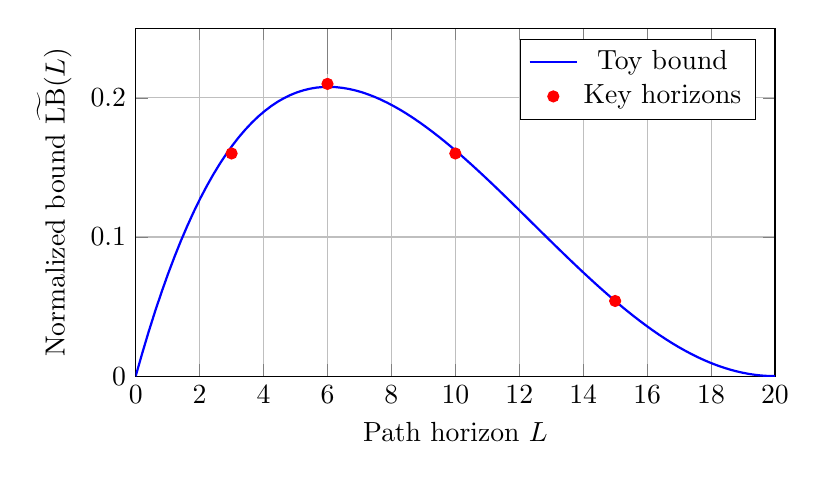
\begin{tikzpicture}
\begin{axis}[
    width=0.8\linewidth,
    height=6cm,
    xlabel={Path horizon $L$},
    ylabel={Normalized bound $\widetilde{\mathrm{LB}}(L)$},
    xmin=0, xmax=20,
    ymin=0, ymax=0.25,
    grid=major,
    legend pos=north east,
]
% Plot the toy function
\addplot[
    domain=0:20,
    samples=100,
    thick,
    blue
] {(1 - exp(-x/6)) * (1 - 0.05*x)^2 / ((1 - 0.05*x)^2 + 1)};

% Mark key points
\addplot[only marks, mark=*, red] coordinates {(3, 0.16) (6, 0.21) (10, 0.16) (15, 0.054)};

% Annotate optimal point
\node[pin={90:{$L_\star \approx 6$}}] at (axis cs:6,0.21) {};

\legend{Toy bound, Key horizons}
\end{axis}
\end{tikzpicture}
\caption{\textbf{Trade-off between path horizon and detection bound (toy model).} 
The normalized lower bound $\widetilde{\mathrm{LB}}(L)$ from 
Equation~\eqref{eq:toy-LB} exhibits a single interior maximum at 
$L_\star \approx 6$, balancing detection power $P_{\mathrm{detect}}(L)$ 
(which increases with $L$) against distortion $\varepsilon(L)$ (which also 
increases with $L$). Parameters: $a=0.05$, $L_0=6$, $\sigma^2=1$.}
\label{fig:path-horizon}
\end{figure}

This example illustrates why the path horizon $L_\star$ should be treated as a tunable parameter
rather than fixed \emph{a priori}: too small and the system misses many events (low
$P_{\mathrm{detect}}$); too large and the geometric approximation degrades (large $\varepsilon(L)$), shrinking
the effective separation and pushing the Davis bound toward vacuity.

\subsection{Guidelines for choosing $\mathcal{P}(L_\star)$ in practice}
\label{subsec:path-guidelines}

We now translate the abstract trade-offs above into concrete guidelines for two representative
domains, using the parameter ranges in Section~\ref{subsec:param-table} as reference.

\paragraph{HERALD-style antigenic drift.}
In HERALD-like settings, a natural path family is the class of mutation paths restricted to
epitope positions:
\[
\mathcal{P}_{\mathrm{HER}}(L)
\;=\;
\Bigl\{ \gamma \text{ induced by at most $L$ single-amino-acid substitutions in a pre-specified
epitope set} \Bigr\}.
\]
Guidelines:
\begin{itemize}[leftmargin=*]
  \item \emph{Start with the biological horizon.} Survey historical antigenic drift to identify the
  typical number of substitutions associated with meaningful immune escape (e.g., 3--10 changes in
  key epitopes over a season). This suggests a plausible range for $L_\star$.

  \item \emph{Audit distortion vs.\ $L$.} For candidate horizons (e.g., $L \in \{3,5,8,10\}$), simulate
  or replay mutational paths in $\mathcal{P}_{\mathrm{HER}}(L)$ and measure empirical distortion
  ratios along each path. Choose $L_\star$ such that
  \[
    \varepsilon(L_\star) \le \varepsilon_{\text{target}},
  \]
  where $\varepsilon_{\text{target}}$ is set by a non-vacuity condition of the form
  $\kappa_{\mathrm{soft}} - 2R \varepsilon(L_\star) > 0$ and by the domain’s tolerance for geometric error.

  \item \emph{Estimate detection power.} Using retrospective data or simulations, estimate
  $P_{\mathrm{detect}}(L)$ as the fraction of historically important trajectories whose relevant
  configuration changes can be realized within $\mathcal{P}_{\mathrm{HER}}(L)$. This empirically populates
  the toy trade-off in~\eqref{eq:toy-LB}.

  \item \emph{Select $L_\star$ via validation.} For each candidate $L$, instantiate the Davis
  system, estimate the components of~\eqref{eq:LB-as-func-of-L} on held-out data (separation
  $\Delta_S(L)$, error terms, coverage), and pick $L_\star$ that maximizes a surrogate of
  $\mathrm{LB}_{\text{Davis}}(L)$ subject to $\varepsilon(L_\star)$ and error-budget constraints.
\end{itemize}

Empirically, horizons in the range $L_\star \approx 5$--$10$ mutations are plausible for seasonal
respiratory viruses, but the framework does not assume any specific value.

\paragraph{VIDAR-style identity dynamics.}
In VIDAR-like settings on $S^{d-1}$, the path family consists of short arcs traced by identity
trajectories:
\[
\mathcal{P}_{\mathrm{VID}}(L)
\;=\;
\Bigl\{ \gamma \text{ with arc length } \ell_g(\gamma) \le L \text{ along an identity trajectory on } S^{d-1} \Bigr\}.
\]
Guidelines:
\begin{itemize}[leftmargin=*]
  \item \emph{Anchor $L$ in typical motion.} Measure frame-to-frame geodesic distances along real
  identity trajectories to estimate typical per-frame angles and the distribution of cumulative arc
  lengths over windows. This yields a natural scale for $L$ (e.g., 0.1--0.5 radians for short clips).

  \item \emph{Check the small-angle regime.} Distortion and the validity of tangent-space
  approximations depend on remaining in a small-angle regime. Distortion audits analogous to
  Section~\ref{subsec:distortion-audits} should verify that $\varepsilon(L)$ remains below a target
  threshold on real trajectories up to $L_\star$.

  \item \emph{Tie to feature behavior.} Evaluate how RIM features (F1--F4) behave as functions of
  $L$; for example, whether subspace leakage (F4) starts to saturate beyond a certain arc length,
  indicating diminishing returns from larger $L$.

  \item \emph{Tune $L_\star$ on validation clips.} As in the HERALD-style case, instantiate the
  Davis system for several candidate $L$ values, estimate the Davis bound components, and pick
  $L_\star$ that balances detection power (ability to see identity anomalies) with geometric fidelity
  and error-budget constraints.
\end{itemize}

In both domains, the key point is that $L_\star$ is not a free, purely heuristic parameter: it is
constrained by distortion audits, margin non-vacuity, and empirical detection power.

\subsection{Limitations of the path-optimization view}
\label{subsec:path-limitations}

The toy analysis above is intentionally simplified. In real systems:

\begin{itemize}[leftmargin=*]
  \item The distortion function $\varepsilon(L)$ may deviate from linearity (e.g., saturating for very
  short paths or accelerating beyond a curvature threshold).

  \item The geodesic separation $\Delta_g(L)$ is not strictly independent of $L$; enlarging
  $\mathcal{P}(L)$ can change which configurations are reachable and how often they occur.

  \item Detection power $P_{\mathrm{detect}}(L)$ is shaped by domain-specific constraints (e.g.,
  epitope masks, occlusions, motion patterns) that may not follow a simple exponential saturation.

  \item Error terms $E_{\mathrm{geom}}(L)$ and $\zeta(L)$ may increase sharply once $L$ crosses a
  regime boundary, making the bound in Theorem~2 vacuous even if separation remains non-zero.

  \item Slices of the data (by demographic, capture condition, or generator family) may exhibit
  different optimal horizons $L_\star$, suggesting that a single global $L_\star$ is suboptimal.
\end{itemize}

For these reasons, Equation~\eqref{eq:toy-LB} should be viewed as a conceptual guide rather than a
prescriptive formula. The practical recommendation is to: (i) parameterize $\mathcal{P}(L)$ in a
domain-appropriate way; (ii) perform distortion audits and feature-behavior checks as $L$ varies;
(iii) estimate the components of the Davis bound on held-out data; and (iv) treat $L_\star$ as a
hyperparameter chosen to maximize a \emph{validated} lower bound, not merely an empirical score.

In summary, path-class design is where geometric theory, domain knowledge, and operational
constraints meet. The Davis framework provides the language and structure for this choice; the
actual selection of $\mathcal{P}(L_\star)$ is an empirical design decision that must be documented,
audited, and revisited as data and deployment conditions evolve.

\section{Operational Protocols and Validation}
\label{sec:ops}
\label{sec:ops-protocols}

Sections~\ref{sec:existence}--\ref{sec:path-optimization} provide the theoretical foundation for Davis systems: existence guarantees from contrastive training and smoothness (Theorem~\ref{thm:existence}), finite-variance detection bounds (Theorem~\ref{thm:davis-main}), and path-horizon optimization. This section translates those results into concrete protocols for building, validating, and monitoring Davis systems in deployment.

The central operational challenge is that all Davis guarantees are \emph{conditional}: they hold only when geometry, features, calibration, and abstention behave as assumed on an in-distribution region $\Omega_{\mathrm{in}}$. In practice, we cannot verify these assumptions exhaustively at training time, nor can we guarantee they persist in deployment. Instead, we must:
\begin{enumerate}[label=(\roman*),leftmargin=*]
  \item \textbf{Audit} the bounded-distortion regime and feature behavior on held-out validation data;
  \item \textbf{Estimate} each component of the error budget $(E_{\mathrm{geom}}, E_{\mathrm{link}}, \xi, \zeta, \delta_{\mathrm{indep}})$ with confidence intervals;
  \item \textbf{Monitor} these quantities during deployment and trigger abstention or retraining when they drift; and
  \item \textbf{Document} all assumptions, thresholds, and procedures in a version-controlled dossier (Section~\ref{sec:discussion}).
\end{enumerate}

This section provides step-by-step protocols for each of these tasks, organized around the error-budget decomposition from Theorem~\ref{thm:davis-main}. Algorithm boxes summarize key procedures; tables provide decision rules; and worked examples show how HERALD and VIDAR instantiate these protocols.

\subsection{Overview: The Validation Workflow}
\label{subsec:ops-overview}

Table~\ref{tab:validation-phases} (conceptual) summarizes the end-to-end validation workflow for a Davis system. The process begins with a trained encoder $f_\theta$ and proceeds through five phases:

\begin{table}[H]
\centering
\caption{\textbf{Davis validation workflow (overview).} Each phase produces estimates or gates that feed into the error budget and abstention policies.}
\label{tab:validation-phases}
\begin{tabularx}{\linewidth}{@{}p{0.18\linewidth}p{0.35\linewidth}p{0.38\linewidth}@{}}
\toprule
\textbf{Phase} & \textbf{Goal} & \textbf{Output} \\
\midrule
1. Distortion audit & Validate $\varepsilon(L_\star) < \varepsilon_{\text{target}}$ on held-out paths & Empirical $\hat\varepsilon(L)$ curve, distortion gate thresholds \\
\addlinespace[2pt]
2. Margin estimation & Verify $\kappa_{\mathrm{soft}} - 2R\hat\varepsilon(L_\star) > 0$ & Estimates $(\hat\kappa_{\mathrm{hard}}, \hat\kappa_{\mathrm{soft}})$ with CIs \\
\addlinespace[2pt]
3. Feature validation & Check monotonicity and linkage on operational range & Feature slopes $\{m_k\}$, linkage failure rate $\hat E_{\mathrm{link}}$ \\
\addlinespace[2pt]
4. Calibration & Fit calibrator and measure ECE/Brier in high-risk region & Calibration map, $\hat\xi$ estimate \\
\addlinespace[2pt]
5. Error budget & Estimate all terms and independence slack & $(\hat E_{\mathrm{geom}}, \hat E_{\mathrm{link}}, \hat\xi, \hat\zeta, \hat\delta_{\mathrm{indep}})$ and vacuity check \\
\bottomrule
\end{tabularx}
\end{table}

\paragraph{Data splits.}
All validation protocols assume access to three disjoint held-out sets:
\begin{itemize}[leftmargin=*]
  \item $\mathcal{D}_{\mathrm{val}}$: primary validation set for distortion audits, margin estimation, and feature checks ($\approx 20\%$ of data);
  \item $\mathcal{D}_{\mathrm{cal}}$: calibration set for fitting the calibrator and estimating $\xi$ ($\approx 10\%$);
  \item $\mathcal{D}_{\mathrm{test}}$: final error-budget estimation and integration test ($\approx 10\%$).
\end{itemize}
These should be stratified by any known slices (demographics, capture conditions, generator families) and temporally separated from training data when time-series structure is present.

\subsection{Phase 1: Distortion Audits}
\label{subsec:distortion-audits}

The bounded-distortion assumption—that Euclidean distances approximate geodesic distances along paths in $\mathcal{P}(L_\star)$ within a factor $(1\pm\varepsilon_\star)$—is the geometric foundation of Davis systems. Distortion audits empirically validate this assumption and identify regimes where it fails.

\subsubsection{Protocol: Measuring Distortion Ratios}

\begin{algorithm}[H]
\caption{Distortion Audit on Validation Paths}
\label{alg:distortion-audit}
\begin{algorithmic}[1]
\Require Encoder $f_\theta$, path family $\mathcal{P}(L)$, validation set $\mathcal{D}_{\mathrm{val}}$
\Ensure Empirical distortion profile $\hat\varepsilon(L)$, per-path distortion ratios $\{\rho_j\}$
\State Sample $N_{\mathrm{path}}$ paths $\{\gamma_j\}_{j=1}^{N_{\mathrm{path}}}$ from $\mathcal{P}(L_\star)$ using $\mathcal{D}_{\mathrm{val}}$
\For{each path $\gamma_j$ with waypoints $(x_{j,1}, \dots, x_{j,T_j})$}
    \State Embed: $z_{j,t} = f_\theta(x_{j,t})$ for $t=1,\dots,T_j$
    \State \textbf{Compute geodesic length:} $\ell_g(\gamma_j) = \sum_{t=1}^{T_j-1} d_g(z_{j,t}, z_{j,t+1})$ \quad \Comment{Using metric $g$}
    \State \textbf{Compute Euclidean length:} $\ell_\delta(\gamma_j) = \sum_{t=1}^{T_j-1} \|z_{j,t} - z_{j,t+1}\|_2$
    \State \textbf{Distortion ratio:} $\rho_j = \ell_\delta(\gamma_j) / \ell_g(\gamma_j)$
\EndFor
\State Compute summary statistics: $\bar\rho = \text{mean}(\rho_j)$, $\sigma_\rho = \text{std}(\rho_j)$, percentiles
\State \textbf{Estimate distortion radius:} $\hat\varepsilon(L_\star) = \max\{|\rho_j - 1|\}$ or $95^{\text{th}}$ percentile of $|\rho_j - 1|$
\State \Return $\hat\varepsilon(L_\star)$, $\{\rho_j\}$, slice-wise breakdowns
\end{algorithmic}
\end{algorithm}

\paragraph{Implementation notes.}
\begin{itemize}[leftmargin=*]
  \item \textbf{Geodesic approximation.} For general pullback manifolds, $d_g(z,z')$ is not available in closed form. Use:
  \begin{itemize}
    \item \emph{Riemannian metric integration}: Numerically integrate $\int \sqrt{g(\dot\gamma,\dot\gamma)}\,dt$ along the path;
    \item \emph{Geodesic solver}: Run a Riemannian optimizer (e.g., using \texttt{geomstats} or \texttt{pymanopt}) to find the shortest path, then measure its length; or
    \item \emph{Inherited geometry}: For hypersphere $\mathbb{S}^{d-1}$ (VIDAR), use $d_g(z,z') = \arccos\langle z,z'\rangle$ directly.
  \end{itemize}
  
  \item \textbf{Path sampling.} Sample paths that reflect operational usage:
  \begin{itemize}
    \item HERALD: mutation trajectories with $\le L_\star$ substitutions in validated epitope positions;
    \item VIDAR: contiguous frame windows of length $T$ with cumulative arc length $\le L_\star$.
  \end{itemize}
  
  \item \textbf{Slice-wise audits.} Compute $\hat\varepsilon(L_\star)$ separately for each slice (e.g., by age group, lighting condition, or generator). Flag slices where $\hat\varepsilon > \varepsilon_{\text{target}}$ for elevated $E_{\mathrm{geom}}$ or mandatory abstention.
\end{itemize}

\subsubsection{Decision Rules and Gates}

\begin{table}[H]
\centering
\caption{\textbf{Distortion audit decision rules.} These thresholds are illustrative; actual values depend on domain and risk tolerance.}
\label{tab:distortion-gates}
\begin{tabularx}{\linewidth}{@{}p{0.22\linewidth}p{0.30\linewidth}p{0.38\linewidth}@{}}
\toprule
\textbf{Condition} & \textbf{Interpretation} & \textbf{Action} \\
\midrule
$\hat\varepsilon(L_\star) < 0.10$ & Low distortion, geometry reliable & Proceed; use geometry-based features (F1--F4 in VIDAR) \\
\addlinespace[2pt]
$0.10 \le \hat\varepsilon(L_\star) < 0.20$ & Moderate distortion & Proceed with caution; down-weight geometric features or widen uncertainty \\
\addlinespace[2pt]
$\hat\varepsilon(L_\star) \ge 0.20$ & High distortion & \textbf{Abstain} or suppress geometry; rely on auxiliary detectors only \\
\addlinespace[2pt]
$|\rho_j - 1| > 0.30$ for $>10\%$ of paths & Frequent outliers & Flag slice for investigation; may indicate OOD inputs or tracking failures \\
\bottomrule
\end{tabularx}
\end{table}

\paragraph{Example (VIDAR on deepfake validation data).}
Suppose Algorithm~\ref{alg:distortion-audit} yields:
\begin{align*}
\bar\rho &= 1.03, \quad \sigma_\rho = 0.08, \\
\hat\varepsilon(L_\star) &= \max_j |\rho_j - 1| = 0.18 \quad \text{(or }95^{\text{th}}\text{ percentile: }0.14\text{)}.
\end{align*}
This suggests moderate distortion. If using the $95^{\text{th}}$ percentile definition, $\hat\varepsilon = 0.14 < 0.20$ and we proceed; if using the max, $\hat\varepsilon = 0.18$ is borderline and we down-weight RIM features or increase abstention thresholds.

\subsection{Phase 2: Margin Estimation and Non-Vacuity}
\label{subsec:margin-estimation}

The configuration margins $(\kappa_{\mathrm{hard}}, \kappa_{\mathrm{soft}})$ from Definition~\ref{def:davis-config} must be empirically validated to ensure that the non-vacuity condition
\[
\kappa_{\mathrm{soft}} - 2R\,\varepsilon(L_\star) \;>\; 0
\]
holds on $\mathcal{D}_{\mathrm{val}}$, where $R$ bounds the geodesic radius of the operational region.

\subsubsection{Protocol: Measuring Configuration Separation}

\begin{algorithm}[H]
\caption{Margin Estimation on Validation Pairs}
\label{alg:margin-estimation}
\begin{algorithmic}[1]
\Require Encoder $f_\theta$, validation set $\mathcal{D}_{\mathrm{val}}$ with coarse labels $Y \in \{0,1\}$
\Ensure Estimates $(\hat\kappa_{\mathrm{hard}}, \hat\kappa_{\mathrm{soft}})$ with confidence intervals
\State Sample $N_{\mathrm{same}}$ same-configuration pairs $(x,x^+)$ with $h(c(f_\theta(x))) = h(c(f_\theta(x^+)))$
\State Sample $N_{\mathrm{diff}}$ different-configuration pairs $(x,x^-)$ with $h(c(f_\theta(x))) \neq h(c(f_\theta(x^-)))$
\State \textbf{Compute distances:}
\State \quad Within-configuration: $\{d_{g^{(0)}_i}\}_{i=1}^{N_{\mathrm{same}}}$ for same-config pairs
\State \quad Across-configuration: $\{d_{g,i}^{(1)}\}_{i=1}^{N_{\mathrm{diff}}}$ for different-config pairs
\State \textbf{Estimate margins:}
\State \quad $\hat\mu_0 = \text{mean}(d_{g,i}^{(0)})$, \quad $\hat\mu_1 = \text{mean}(d_{g,i}^{(1)})$
\State \quad $\hat\Delta_g = \hat\mu_1 - \hat\mu_0$
\State \quad $\hat\kappa_{\mathrm{hard}} = \hat\mu_0 + 2\hat\sigma_0$ \quad \Comment{Conservative: mean + 2 std of within-config}
\State \quad $\hat\kappa_{\mathrm{soft}} = \hat\mu_1 - 2\hat\sigma_1$ \quad \Comment{Conservative: mean - 2 std of across-config}
\State Compute bootstrap CIs for $(\hat\kappa_{\mathrm{hard}}, \hat\kappa_{\mathrm{soft}})$ via resampling
\State \textbf{Non-vacuity check:} Verify $\hat\kappa_{\mathrm{soft}} - 2R\,\hat\varepsilon(L_\star) > 0$ using $\hat\varepsilon$ from Phase~1
\State \Return $(\hat\kappa_{\mathrm{hard}}, \hat\kappa_{\mathrm{soft}})$, CIs, non-vacuity flag
\end{algorithmic}
\end{algorithm}

\paragraph{Interpretation.}
If $\hat\kappa_{\mathrm{hard}} < \hat\kappa_{\mathrm{soft}}$ and the non-vacuity condition holds, the system has a validated ambiguity band $[\hat\kappa_{\mathrm{hard}}, \hat\kappa_{\mathrm{soft}}]$ where abstention should trigger. If $\hat\kappa_{\mathrm{hard}} \ge \hat\kappa_{\mathrm{soft}}$ or non-vacuity fails, the configuration structure is not sufficiently separated for reliable detection at horizon $L_\star$; either reduce $L_\star$, increase $\lambda$ (smoothness), or collect more contrastive training data.

\subsection{Phase 3: Error Budget Estimation}
\label{subsec:error-budget-estimation}

The compositional guarantee in Theorem~\ref{thm:davis-main} decomposes correctness into four error terms plus an independence slack. This subsection provides estimation protocols for each.

\subsubsection{Geometry Error ($E_{\mathrm{geom}}$)}
\label{subsubsec:egeom}

\emph{Definition.} $E_{\mathrm{geom}}$ is the probability that the Davis manifold geometry behaves outside its validated regime in a way that materially corrupts the detection statistic $S$.

\paragraph{Operational proxy.}
On $\mathcal{D}_{\mathrm{test}}$, flag samples as geometry failures if:
\begin{enumerate}[label=(\alph*),leftmargin=*]
  \item Any path $\gamma$ used to compute features has distortion $|\rho_\gamma - 1| > \varepsilon_{\text{max}}$ (e.g., $\varepsilon_{\text{max}} = 0.25$);
  \item Smoothness checks fail (e.g., large second-order finite differences in embeddings suggest high local curvature); or
  \item Paths exit the validated region (e.g., geodesic distance to training support exceeds a Mahalanobis threshold).
\end{enumerate}

\paragraph{Estimator.}
\[
\hat E_{\mathrm{geom}}
\;=\;
\frac{1}{N_{\mathrm{test}}} \sum_{i=1}^{N_{\mathrm{test}}} \mathbb{1}\{\text{sample } i \text{ flagged as geometry failure}\}.
\]
Compute separately on slices and worst-case across slices for a conservative bound.

\subsubsection{Linkage Error ($E_{\mathrm{link}}$)}
\label{subsubsec:elink}

\emph{Definition.} $E_{\mathrm{link}}$ is the probability that features fail to track geodesic distance even when geometry is good—e.g., monotonicity breaks, PIT nulls are misspecified, or feature fusion produces a statistic $S$ uncorrelated with true configuration change.

\paragraph{Operational proxy.}
On $\mathcal{D}_{\mathrm{test}}$, restrict to samples passing geometry checks (not flagged in Phase~1). For each, compute:
\begin{enumerate}[label=(\alph*),leftmargin=*]
  \item Ground-truth configuration change $\Delta c$ (binary: same vs. different);
  \item Predicted statistic $S$ and its sign relative to threshold $s_\star$.
\end{enumerate}
Flag as linkage failures any samples where $S$ and $\Delta c$ are anti-correlated (e.g., $S < s_\star$ but $\Delta c = 1$, or vice versa) despite passing geometry gates.

\paragraph{Estimator.}
\[
\hat E_{\mathrm{link}}
\;=\;
\frac{\#\{\text{samples with anti-correlated }(S, \Delta c)\}}{\#\{\text{samples passing geometry checks}\}}.
\]

\subsubsection{Calibration Error ($\xi$)}
\label{subsubsec:xi}

\emph{Definition.} $\xi$ quantifies miscalibration in the mapping from the raw statistic $S$ to the calibrated probability $\hat p = \text{calib}(S)$ in the high-risk region ($S > s_\star$).

\paragraph{Protocol: Expected Calibration Error (ECE).}
\begin{enumerate}[label=\arabic*.,leftmargin=*]
  \item Fit a calibrator (e.g., isotonic regression, Platt scaling, or temperature scaling) on $\mathcal{D}_{\mathrm{cal}}$ to map $S \to \hat p$.
  \item On $\mathcal{D}_{\mathrm{test}}$, bin samples by $\hat p$ (e.g., 10 bins from 0 to 1).
  \item For each bin $B_k$ in the high-risk region ($\hat p > 0.5$ or $S > s_\star$), compute:
  \[
  \text{ECE}_k
  \;=\;
  \bigl|\text{avg. predicted } \hat p \text{ in bin} - \text{fraction of true positives in bin}\bigr|.
  \]
  \item Set $\hat\xi = \max_k \text{ECE}_k$ over high-risk bins, or use a weighted average.
\end{enumerate}

\paragraph{Alternative: Brier score decomposition.}
Decompose the Brier score restricted to $S > s_\star$ into calibration and refinement components; use the calibration component as $\hat\xi$.

\subsubsection{Abstention Failure ($\zeta$)}
\label{subsubsec:zeta}

\emph{Definition.} $\zeta$ is the probability that the system fails to abstain when it should—i.e., issues a non-abstaining prediction (`\texttt{info}', `\texttt{warn}', or `\texttt{high\_risk}') despite being out-of-regime.

\paragraph{Operational proxy.}
Define an \emph{oracle abstention set} $\mathcal{A}_{\text{oracle}}$ on $\mathcal{D}_{\mathrm{test}}$ as samples that fail any of:
\begin{itemize}[leftmargin=*]
  \item Distortion gate ($|\rho| - 1 > \varepsilon_{\text{max}}$);
  \item Margin check ($d_g \in [\kappa_{\mathrm{hard}}, \kappa_{\mathrm{soft}}]$, i.e., in ambiguous band);
  \item Feature range check ($S$ or individual features outside $[F_{\min}, F_{\max}]$ from training);
  \item Support check (e.g., Mahalanobis distance to training manifold exceeds threshold).
\end{itemize}

Let $\mathcal{A}_{\text{pred}}$ be the set of samples for which the Davis system actually abstains. Then:
\[
\hat\zeta
\;=\;
\frac{\#\bigl(\mathcal{A}_{\text{oracle}} \setminus \mathcal{A}_{\text{pred}}\bigr)}{\#\mathcal{A}_{\text{oracle}}}
\;=\;
\frac{\text{should-abstain but didn't}}{\text{total should-abstain}}.
\]

\subsubsection{Independence Slack ($\delta_{\mathrm{indep}}$)}
\label{subsubsec:deltaindep}

\emph{Definition.} $\delta_{\mathrm{indep}}$ captures the excess probability that \emph{some} error occurs beyond what would be predicted by assuming $(E_{\mathrm{geom}}, E_{\mathrm{link}}, \xi, \zeta)$ are independent.

\paragraph{Estimator.}
On $\mathcal{D}_{\mathrm{test}}$, flag each sample for each error type. Compute:
\begin{align*}
\hat\varepsilon_{\text{joint}}
&= \frac{\#\{\text{samples with } \ge 1 \text{ error}\}}{N_{\mathrm{test}}}, \\
\hat\varepsilon_{\text{mult}}
&= 1 - (1-\hat E_{\mathrm{geom}})(1-\hat E_{\mathrm{link}})(1-\hat\xi)(1-\hat\zeta).
\end{align*}
Then:
\[
\hat\delta_{\mathrm{indep}}
\;=\;
\max\bigl\{0,\, \hat\varepsilon_{\text{joint}} - \hat\varepsilon_{\text{mult}}\bigr\}.
\]
If $\hat\delta_{\mathrm{indep}} > 0.1$, the multiplicative bound is optimistic and a union-bound fallback should be used.

\subsection{Phase 4: Abstention and Quality Gates}
\label{subsec:abstention-gates}

Abstention in Davis systems is not a post-hoc confidence threshold; it is a first-class outcome triggered when assumptions fail. This subsection formalizes abstention policies.

\subsubsection{Multi-Stage Abstention Architecture}

\begin{table}[H]
\centering
\caption{\textbf{Abstention gates and decision logic.} Gates are applied sequentially; failure at any stage triggers `\texttt{insufficient\_signal}'.}
\label{tab:abstention-gates}
\begin{tabularx}{\linewidth}{@{}p{0.16\linewidth}p{0.35\linewidth}p{0.40\linewidth}@{}}
\toprule
\textbf{Gate} & \textbf{Condition} & \textbf{Interpretation} \\
\midrule
G1: Quality & Basic quality checks (resolution, blur, completeness) & Filters obviously broken inputs \\
\addlinespace[2pt]
G2: OOD & Mahalanobis distance, reconstruction error, or novelty score & Detects inputs far from training support \\
\addlinespace[2pt]
G3: Distortion & $|\rho_\gamma - 1| \le \varepsilon_{\max}$ for all paths $\gamma$ & Ensures bounded-distortion regime \\
\addlinespace[2pt]
G4: Margin & $d_g \notin [\kappa_{\mathrm{hard}}, \kappa_{\mathrm{soft}}]$ & Avoids ambiguous band \\
\addlinespace[2pt]
G5: Feature range & All features $F_k \in [F_{\min}^{(k)}, F_{\max}^{(k)}]$ & Checks features are in-range \\
\addlinespace[2pt]
G6: Vacuity & $\hat E_{\mathrm{geom}} + \hat E_{\mathrm{link}} + \hat\xi + \hat\zeta < \tau_{\mathrm{vac}}$ & Global error budget below vacuity threshold \\
\bottomrule
\end{tabularx}
\end{table}

\paragraph{Decision tree.}
\begin{enumerate}[label=\arabic*.,leftmargin=*]
  \item If any of G1--G5 fail for a sample, output `\texttt{insufficient\_signal}'.
  \item If G6 fails (error budget exceeds $\tau_{\mathrm{vac}} \approx 0.7$), downgrade all alerts or abstain globally.
  \item Otherwise, compute $S$ and proceed to threshold-based decisions: `\texttt{info}', `\texttt{warn}', or `\texttt{high\_risk}'.
\end{enumerate}

\subsection{Phase 5: Calibration Methods}
\label{subsec:calibration-methods}

Calibration maps the raw detection statistic $S$ to a probability $\hat p \approx \mathbb{P}(Y=1 \mid S)$. This subsection describes three common approaches.

\subsubsection{Isotonic Regression (Non-Parametric)}

Fit a piecewise-constant, monotone map $S \mapsto \hat p$ via isotonic regression on $\mathcal{D}_{\mathrm{cal}}$. This preserves the ranking of $S$ while adjusting probabilities to match empirical frequencies.

\paragraph{Advantages:} Flexible, no parametric assumptions.

\paragraph{Disadvantages:} Can overfit on small calibration sets; requires careful binning.

\subsubsection{Platt Scaling (Logistic)}

Fit a logistic model:
\[
\hat p(S) = \frac{1}{1 + \exp(-a S - b)},
\]
where $(a,b)$ are learned on $\mathcal{D}_{\mathrm{cal}}$ via maximum likelihood.

\paragraph{Advantages:} Simple, interpretable, works well when $S$ is approximately linear in log-odds.

\paragraph{Disadvantages:} Assumes a specific functional form.

\subsubsection{Temperature Scaling (Neural)}

If $S$ is the output of a neural network before softmax, add a learned temperature $T>0$:
\[
\hat p(S) = \frac{\exp(S/T)}{\exp(S/T) + 1}.
\]
Fit $T$ on $\mathcal{D}_{\mathrm{cal}}$ to minimize negative log-likelihood.

\paragraph{Recommendation.}
Use isotonic regression by default for Davis systems; fall back to Platt or temperature scaling if the calibration set is small ($<1000$ samples).

\subsection{Validation Checklists and Monitoring}
\label{subsec:validation-checklists}

\begin{mdframed}[linewidth=0.5pt,backgroundcolor=black!1]
\noindent\textbf{Pre-Deployment Checklist}
\begin{enumerate}[leftmargin=*,itemsep=2pt]
  \item[$\square$] Distortion audit complete: $\hat\varepsilon(L_\star) < \varepsilon_{\text{target}}$ on all validated slices
  \item[$\square$] Margins verified: $\hat\kappa_{\mathrm{soft}} - 2R\hat\varepsilon(L_\star) > 0$ with CIs
  \item[$\square$] Error budget estimated: $(\hat E_{\mathrm{geom}}, \hat E_{\mathrm{link}}, \hat\xi, \hat\zeta, \hat\delta_{\mathrm{indep}})$ documented
  \item[$\square$] Vacuity check: $\hat E_{\mathrm{geom}} + \hat E_{\mathrm{link}} + \hat\xi + \hat\zeta < \tau_{\mathrm{vac}}$
  \item[$\square$] Calibration validated: ECE $< 0.05$ in high-risk region on $\mathcal{D}_{\mathrm{test}}$
  \item[$\square$] Abstention gates tested: $\hat\zeta < 0.05$ on oracle abstention set
  \item[$\square$] Slice-wise audits: No slice has $\hat\varepsilon > 1.5 \times \varepsilon_{\text{target}}$ or $\hat E_{\text{sum}} > \tau_{\mathrm{vac}}$
  \item[$\square$] Davis dossier prepared: All thresholds, data splits, and procedures version-controlled
\end{enumerate}
\end{mdframed}

\subsubsection{Deployment Monitoring}

Once deployed, Davis systems require continuous monitoring to detect distributional drift. Recommended metrics (computed on rolling windows, e.g., weekly):

\begin{table}[H]
\centering
\caption{\textbf{Deployment monitoring dashboard (recommended metrics).}}
\label{tab:monitoring-dashboard}
\begin{tabularx}{\linewidth}{@{}p{0.25\linewidth}p{0.68\linewidth}@{}}
\toprule
\textbf{Metric} & \textbf{Trigger Condition for Re-Audit} \\
\midrule
Abstention rate & $>20\%$ increase vs. validation baseline \\
Distortion $\hat\varepsilon(L)$ & Mean or $95^{\text{th}}$ percentile exceeds $1.2 \times \varepsilon_{\text{target}}$ \\
Feature statistics & Drift in $\mathbb{E}[F_k]$ or $\text{Var}(F_k)$ beyond 2 std from validation \\
Calibration drift & ECE increases by $>0.03$ in high-risk region \\
Slice imbalance & Any slice has abstention rate $>2\times$ global rate \\
Error budget & $\hat E_{\text{sum}}$ exceeds $0.8 \times \tau_{\mathrm{vac}}$ (warning) or $\tau_{\mathrm{vac}}$ (halt) \\
\bottomrule
\end{tabularx}
\end{table}

\paragraph{Response to drift.}
When monitoring triggers indicate assumption violations:
\begin{enumerate}[label=(\alph*),leftmargin=*]
  \item \textbf{Minor drift}: Widen uncertainty, increase abstention thresholds, flag affected slices.
  \item \textbf{Moderate drift}: Pause high-risk alerts; rerun Phases 1--5 on recent data; update dossier.
  \item \textbf{Severe drift}: Halt deployment; retrain encoder with updated $\lambda$ or path family; restart validation from Phase~1.
\end{enumerate}

\subsection{Computational Considerations}
\label{subsec:computational-ops}

Davis systems trade off geometric fidelity for computational cost. This subsection quantifies typical overheads.

\subsubsection{Training-Time Costs}

\begin{table}[H]
\centering
\caption{\textbf{Computational overhead of Davis construction (training).} Relative to baseline contrastive training without smoothness regularization.}
\label{tab:training-costs}
\begin{tabularx}{\linewidth}{@{}p{0.28\linewidth}p{0.30\linewidth}p{0.33\linewidth}@{}}
\toprule
\textbf{Component} & \textbf{Overhead Factor} & \textbf{Notes} \\
\midrule
Jacobian regularization & $1.5\times$--$3\times$ & Forward and backward for $\nabla_x f_\theta$ \\
Laplacian regularization & $2\times$--$5\times$ & Requires graph construction + sparse linear algebra \\
Distortion audits (validation) & $0.1\times$--$0.3\times$ per epoch & Geodesic integration on sampled paths \\
\bottomrule
\end{tabularx}
\end{table}

\paragraph{Mitigation strategies.}
\begin{itemize}[leftmargin=*]
  \item Use stochastic Jacobian estimation (random projections) instead of full Hessian.
  \item Run distortion audits asynchronously during training; cache geodesic computations.
  \item For frozen backbones (inherited margin), smoothness regularization is unnecessary.
\end{itemize}

\subsubsection{Inference-Time Costs}

\begin{table}[H]
\centering
\caption{\textbf{Runtime overhead of Davis inference.} Per-sample latency relative to a single forward pass.}
\label{tab:inference-costs}
\begin{tabularx}{\linewidth}{@{}p{0.28\linewidth}p{0.30\linewidth}p{0.33\linewidth}@{}}
\toprule
\textbf{Operation} & \textbf{Overhead Factor} & \textbf{Notes} \\
\midrule
Embedding ($f_\theta$) & $1\times$ & Baseline \\
Path features (F1--F4) & $0.5\times$--$1\times$ & Geodesic differences, tangent projections \\
Distortion check & $0.2\times$--$0.5\times$ & If geodesic solver used; negligible for hypersphere \\
PIT normalization & $0.1\times$ & ECDF lookups \\
Calibration map & $0.05\times$ & Isotonic or logistic eval \\
\midrule
\textbf{Total} & $\mathbf{2\times}$--$\mathbf{3\times}$ & Acceptable for offline/forensic use \\
\bottomrule
\end{tabularx}
\end{table}

\paragraph{Optimization.}
For real-time applications:
\begin{itemize}[leftmargin=*]
  \item Precompute null CDFs for PIT offline.
  \item Use closed-form geodesics (e.g., $\mathbb{S}^{d-1}$) to avoid iterative solvers.
  \item Cache embeddings for multi-frame or temporal inputs.
\end{itemize}

\subsection{Worked Example: VIDAR Validation Protocol}
\label{subsec:vidar-example}

To make the protocols concrete, we sketch how VIDAR (deepfake detection via identity dynamics) instantiates Phases 1--5.

\paragraph{Phase 1: Distortion audit.}
\begin{enumerate}[label=\arabic*.,leftmargin=*]
  \item Sample $N_{\mathrm{path}} = 500$ short talking-head clips (real and synthetic) from $\mathcal{D}_{\mathrm{val}}$.
  \item Extract ArcFace embeddings $\{f_\theta(x_t)\}$ for frames $t=1,\dots,T$.
  \item Normalize to $\mathbb{S}^{d-1}$; compute geodesic arc length $\ell_g = \sum_t \arccos\langle f_t, f_{t+1}\rangle$.
  \item Compute Euclidean chord length $\ell_\delta = \sum_t \|f_t - f_{t+1}\|_2$.
  \item Measure $\rho_j = \ell_\delta / \ell_g$ for each clip $j$; compute $\hat\varepsilon = 95^{\text{th}}$ percentile of $|\rho_j - 1|$.
  \item Result: $\hat\varepsilon(L_\star=0.3\text{ rad}) = 0.12$ (acceptable; proceed).
\end{enumerate}

\paragraph{Phase 2: Margin estimation.}
\begin{enumerate}[label=\arabic*.,leftmargin=*]
  \item Sample pairs: same-identity clips from $\mathcal{D}_{\mathrm{val}}$ (real), different-identity clips (real vs. synthetic or different people).
  \item Compute geodesic distances $d_g$ between mean embeddings per clip.
  \item Fit: $\hat\kappa_{\mathrm{hard}} = 0.08\text{ rad}$, $\hat\kappa_{\mathrm{soft}} = 0.18\text{ rad}$.
  \item Non-vacuity: $0.18 - 2(0.5)(0.12) = 0.18 - 0.12 = 0.06 > 0$ .
\end{enumerate}

\paragraph{Phase 3: Error budget.}
\begin{itemize}[leftmargin=*]
  \item $\hat E_{\mathrm{geom}} = 0.08$ (8\% of clips have $|\rho| > 0.20$; flagged)
  \item $\hat E_{\mathrm{link}} = 0.05$ (5\% anti-correlation between RIM features and labels)
  \item $\hat\xi = 0.04$ (ECE in high-risk region)
  \item $\hat\zeta = 0.03$ (3\% fail to abstain when they should)
  \item $\hat\delta_{\mathrm{indep}} = 0.02$ (joint vs. multiplicative slack)
\end{itemize}
Sum: $0.08 + 0.05 + 0.04 + 0.03 = 0.20 < \tau_{\mathrm{vac}} = 0.70$ .

\paragraph{Phase 4: Abstention gates.}
Configure gates G1--G5 with thresholds: quality (blur $< 0.3$), OOD (Mahalanobis $< 3.0$), distortion ($|\rho| < 0.20$), margin ($d_g \notin [0.08, 0.18]$), feature range (all RIM features in $[-3,3]$ after PIT).

\paragraph{Phase 5: Calibration.}
Fit isotonic regression on $\mathcal{D}_{\mathrm{cal}}$ mapping $S \to \hat p$; validate ECE $= 0.035 < 0.05$.

\paragraph{Outcome.}
VIDAR passes all validation checks and can deploy with the stated error budget. During deployment, monitor $\hat\varepsilon$, abstention rate, and ECE weekly; retrain if any drift beyond thresholds in Table~\ref{tab:monitoring-dashboard}.

\subsection{Summary and Transition to Discussion}

This section has translated the theoretical Davis framework into actionable protocols:
\begin{itemize}[leftmargin=*]
  \item Algorithm~\ref{alg:distortion-audit} and~\ref{alg:margin-estimation} validate geometry and configuration structure.
  \item Subsection~\ref{subsec:error-budget-estimation} provides estimation recipes for each error-budget component.
  \item Tables~\ref{tab:distortion-gates},~\ref{tab:abstention-gates}, and~\ref{tab:monitoring-dashboard} give decision rules and monitoring triggers.
  \item The VIDAR example (Subsection~\ref{subsec:vidar-example}) demonstrates end-to-end instantiation.
\end{itemize}

These protocols are not optional hygiene; they are the \emph{enabling condition} for Theorem~\ref{thm:davis-main}. Without empirical validation of bounded distortion, non-vacuous margins, and sub-threshold error budgets, the compositional lower bound is vacuous and Davis guarantees do not apply. Section~\ref{sec:discussion} now examines when these conditions hold in practice, discusses failure modes, and outlines the broader research agenda for geometry-first detection systems.

\section{Discussion and Outlook}
\label{sec:discussion}

Figure~\ref{fig:davis-roadmap} summarizes the Davis construction--traversal--guarantee pipeline: we
(1) learn a Riemannian manifold and path family on which geodesic distance has semantic meaning;
(2) traverse that geometry at runtime using Euclidean surrogates within a bounded-distortion regime;
and (3) attach finite-variance, compositional error bounds and abstention policies that make the
resulting system falsifiable.

\begin{figure}[t]
  \centering
  % \includegraphics[width=\linewidth]{fig_davis_roadmap.pdf}
  \caption{Davis roadmap (conceptual). \emph{Top:} construction phase---contrastive and
  smoothness-regularized training produces a pullback manifold $(\mathcal{M},g)$, a benign path family
  $\mathcal{P}(L_\star)$, and configuration structure with hard/soft margins and an ambiguity band.
  \emph{Middle:} traversal phase---runtime observations $x$ are embedded, paths are formed, features
  are extracted and PIT-normalized, and a scalar statistic $S$ is computed with abstention gates.
  \emph{Bottom:} theory---Theorem~\ref{thm:existence} ensures the existence of a Davis manifold
  under InfoNCE + smoothness; Theorem~\ref{thm:davis-main} provides a finite-variance detection
  bound with a compositional error budget; Section~\ref{sec:path-optimization} discusses how to
  select an operational path horizon $L_\star$. HERALD and VIDAR (Tables~\ref{tab:herald-davis} and~\ref{tab:vidar-davis}) instantiate this pipeline in virology and video forensics.}
  \label{fig:davis-roadmap}
\end{figure}

\subsection{Why Geometry?}

Davis systems are built on a geometry-first view: we posit that the right notion of ``distance'' for a
given domain lives on a curved functional state space, not in the raw observation coordinates. This
choice is motivated by four recurring observations across domains.

\paragraph{Identity-preserving dynamics live on low-curvature manifolds.}
In HERALD, sequences that differ by a small number of epitope mutations induce nearby points
and short geodesics on an antigenic manifold. In VIDAR, embeddings from a face-recognition
backbone lie on a hypersphere, and clips induce identity trajectories with constrained velocity and
curvature. In both cases, real-world dynamics respect continuity constraints that make a
Riemannian description natural.

\paragraph{Bounded distortion makes Euclidean computations meaningful.}
Section~\ref{sec:existence} shows that contrastive training plus smoothness regularization yield a
pullback metric $g$ whose geodesics are well-approximated by straight chords over path families
$\mathcal{P}(L_\star)$, with distortion controlled by $\varepsilon(L_\star)$. This lets us work with
Euclidean distances and tangent-space statistics in practice while retaining a geometric
interpretation: we know \emph{where} those approximations are valid, and by how much they may
distort.

\paragraph{Trajectories expose failures earlier than snapshots.}
High-risk events in Davis systems are typically \emph{path properties}: a variant crossing an antigenic
margin, an identity trajectory leaving a plausible band, a control policy departing a safe
region. Representing observations as paths on $(\mathcal{M},g)$ makes it natural to talk about
velocity, curvature, and subspace leakage---and to detect abnormal behavior even when individual
observations look unremarkable.

\paragraph{Geometry is where assumptions live.}
The bounded-distortion regime, margin non-vacuity
$\kappa_{\mathrm{soft}} - 2R\varepsilon(L_\star) > 0$, and path-family
constraints are all geometric assumptions. By stating them explicitly on $(\mathcal{M},g)$ and
auditing them via distortion checks and margin measurements, we get falsifiable guarantees:
when the geometry drifts or the path regime is violated, we know the theory no longer applies and
must abstain or retrain.

\subsection{When the Theory Applies---and When to Abstain}

Section~\ref{sec:existence} (Theorem~\ref{thm:existence}) and
Section~\ref{sec:theory2} (Theorem~\ref{thm:davis-main}) are deliberately conditional. In practice,
the Davis guarantees are intended to apply on a validated region
$\mathcal{R}_{\mathrm{valid}} \subseteq \mathcal{X}$ of in-distribution inputs where four conditions hold.

\medskip\noindent
\textbf{(T1) Geometry is stable.} Distortion audits (Section~\ref{sec:ops-protocols}) show that along
benign paths in $\mathcal{P}(L_\star)$, the ratio $\delta/d_g$ concentrates near~1 with tails bounded
by a pre-registered $\varepsilon_\star$, and that temporal smoothness assumptions used in
feature design are empirically satisfied.

\medskip\noindent
\textbf{(T2) Configurations are separated.} Validation data support a positive gap between
configurations that coarse labels $h$ map to~0 vs.~1, after accounting for distortion:
$\kappa_{\mathrm{soft}} - 2R\varepsilon(L_\star) > 0$. In HERALD this appears as separation
between vaccine-like and escape-like clusters in antigenic space; in VIDAR as a gap between
same-identity and different-identity arcs on the hypersphere.

\medskip\noindent
\textbf{(T3) Features track geometry.} The path features and aggregated statistic $S$ satisfy a
monotone linkage $\Delta_S \ge g(\Delta_g)$ on an empirically verified operational range, with
non-trivial separation $\Delta_S > 0$ and finite second moments. Outside that range, the system
either treats features as OOD or down-weights their contribution.

\medskip\noindent
\textbf{(T4) Calibration and abstention behave as specified.} Calibration error in the high-risk
region is bounded by $\xi$, and abstention failure by $\zeta$, with both terms estimated under the
protocols of Section~\ref{sec:ops-protocols}. The error budget
$E_{\mathrm{geom}} + E_{\mathrm{link}} + \xi + \zeta$ stays below a pre-registered vacuity threshold
$\tau_{\mathrm{vac}}$ on the deployment distribution.

\begin{mdframed}
\textbf{Design principle.} When empirical audits suggest that (T1)--(T4) may not hold on a slice or
deployment---e.g., distortion tails are heavy, margins collapse, or calibration drifts---a Davis system
should \emph{increase abstention} rather than lowering thresholds to maintain apparent coverage.
\end{mdframed}

Outside $\mathcal{R}_{\mathrm{valid}}$ the finite-variance Cantelli bound may be loose and the compositional
guarantee in Theorem~\ref{thm:davis-main} may become vacuous. The intended response is not to
interpret the bound optimistically, but to treat such regimes as unvalidated: widen uncertainty,
rely on external checks, or defer to human or laboratory adjudication.

\subsection{Limitations and Failure Modes}

Davis systems have several structural limitations.

\paragraph{Locality of the bounded-distortion regime.}
The distortion bounds in Section~\ref{sec:existence} are local in path length: they apply along
paths in $\mathcal{P}(L)$ with $L \le L_\star$ and bounded curvature. Recombination events, hard
scene cuts, sudden lighting changes, or control discontinuities can produce large geodesic jumps
where linearization fails. In such regimes the distinction between geodesic and Euclidean distance
matters, and Davis guarantees should not be applied.

\paragraph{Dependence on the backbone.}
The geometry is induced by a particular encoder $f_\theta$. If $f_\theta$ is biased or brittle---for
example, face embeddings that compress distances for underrepresented groups, or sequence
embeddings that collapse in novel lineages---then the Davis manifold inherits those failures.
Conditions on the inherited margin (e.g., Assumption~A5') must be checked slice-wise, not assumed.

\paragraph{Heavy-tailed noise and finite-variance bounds.}
The use of Cantelli's inequality in Theorem~\ref{thm:davis-main} buys generality (finite second
moments suffice) at the cost of slower tail decay. In strongly heavy-tailed settings, the resulting
bounds may be numerically weak. Sub-exponential or sub-Weibull refinements are an open direction
(Section~\ref{subsec:open-problems}).

\paragraph{Correlated failures.}
The multiplicative form of the bound assumes approximate independence among
geometry, linkage, calibration, and abstention errors. When these error sources share common
causes---for example, high curvature simultaneously degrading distortion and feature monotonicity,
or OOD inputs breaking geometry and calibration together---the independence slack
$\delta_{\mathrm{indep}}$ can be large and the multiplicative bound optimistic; the union bound
fallback becomes appropriate but may be vacuous.

\paragraph{Computational cost.}
Smoothness regularization, Jacobian penalties, and geodesic approximations can be substantially
more expensive than training a black-box encoder with a simple loss. Runtime monitoring and
distortion audits add overhead. For offline or forensic settings this cost may be acceptable; for
real-time, high-throughput applications it can be a limiting factor.

\paragraph{Red flags.}
Empirically, the following are warning signs that a Davis instantiation is out of its validated regime:
(i) distortion audits show large $\varepsilon(L_\star)$ or heavy tails, but coverage remains high;
(ii) measured separation $\Delta_S$ collapses on deployment data; (iii) the estimated error budget
exceeds $\tau_{\mathrm{vac}}$; or (iv) slice analyses show severe disparities that cannot be explained by
data scarcity alone.

\subsection{Relation to Existing Frameworks}

Davis manifolds touch several established areas: metric learning, Riemannian machine learning,
conformal prediction and selective classification, and domain-specific geometric systems such as
HERALD and VIDAR. Table~\ref{tab:relation-prior-work} summarizes the relationship at a high
level.

\begin{table}[H]
  \centering
  \begin{tabularx}{\linewidth}{@{}p{0.20\linewidth}p{0.32\linewidth}X@{}}
    \toprule
    \textbf{Framework} & \textbf{Primary focus} & \textbf{What Davis manifolds add} \\
    \midrule
    Metric / contrastive learning &
    Embeddings where similar pairs are close, dissimilar pairs are far &
    Explicit Riemannian structure, bounded-distortion path families, and soft/hard configuration margins with ambiguity bands. \\
    \addlinespace
    Riemannian ML (SPD nets, hyperbolic embeddings, etc.) &
    Optimization and representation on fixed manifolds &
    Data-driven \emph{construction} of the manifold via pullback metrics, plus deployment-time distortion audits and abstention policies tied to the geometry. \\
    \addlinespace
    Conformal / selective prediction, OOD detection &
    Coverage guarantees, abstention, uncertainty quantification &
    A geometric substrate that specifies when abstention should trigger (e.g., distortion or margin violations), and a compositional error budget that includes geometry and feature linkage. \\
    \addlinespace
    HERALD, VIDAR (domain-specific systems) &
    Viral surveillance and deepfake forensics with geometry-based detectors &
    A unifying abstraction: both are instances of Davis systems with problem-specific manifolds, path families, and statistics; the present work generalizes their theory and operational protocols. \\
    \bottomrule
  \end{tabularx}
  \caption{Relation between Davis manifolds and selected prior frameworks.}
  \label{tab:relation-prior-work}
\end{table}

Davis manifolds can be seen as an interface layer: metric learning and Riemannian ML supply
tools for constructing $(\mathcal{M},g)$; conformal prediction and selective classification supply tools
for abstention and coverage; and domain knowledge supplies task-specific path families, configuration
maps, and features.

\subsection{The Davis Universality Conjecture}

A central motivating question is whether Davis manifolds capture a broad class of safety-relevant
temporal problems.

\begin{quote}
\textbf{Conjecture (Davis universality).}%
\quad
Any supervised learning problem with identity-preserving temporal structure can be recast as path
classification on a Davis manifold, provided that:
\begin{enumerate}[label=(U\arabic*), topsep=2pt,leftmargin=1.5em]
  \item there exists an appropriate notion of ``identity'' or functional state that evolves continuously
        along benign trajectories;
  \item a contrastive signal (same/different or similar/dissimilar pairs) is available to learn or validate
        a separation margin;
  \item smoothness can be incentivized architecturally or via regularization so that bounded-distortion
        path families exist; and
  \item configuration changes of interest exhibit a positive geodesic jump (a margin $\kappa > 0$)
        in the learned geometry.
\end{enumerate}
Under these conditions, there exists a Davis manifold and path family for which the detection task
can be formulated as classifying paths that cross configuration margins.
\end{quote}

This conjecture may not hold in full generality, but it provides a concrete research program: identify
domains that satisfy (or fail) the conditions, characterize what identity and smoothness mean in
each, and study how far the Davis construction can be pushed.

\medskip\noindent
\emph{Examples likely to satisfy (U1)--(U4).}
\begin{itemize}[leftmargin=1.6em,itemsep=2pt,topsep=2pt]
  \item Protein or viral evolution (identity = functional antigenic state; paths = mutation trajectories).
  \item Video-based identity or pose tracking (identity = person or object; paths = short clips).
  \item Robot or autonomous-vehicle telemetry (identity = system state; paths = control trajectories).
  \item Speaker or instrument recognition over time (identity = source; paths = audio segments).
\end{itemize}

\noindent
\emph{Examples that may violate the conjecture.}
\begin{itemize}[leftmargin=1.6em,itemsep=2pt,topsep=2pt]
  \item Domains with rapidly mixing Markov dynamics and no meaningful notion of identity
        (violating (U1)).
  \item Settings where contrastive labels are unavailable or untrustworthy (violating (U2)).
  \item Adversarial environments that routinely induce discontinuous jumps in the relevant state,
        or where the generator explicitly targets the distortion and margin regimes (violating (U3)
        and (U4)).
\end{itemize}

\subsection{Open Problems}
\label{subsec:open-problems}

Several technical questions are left intentionally open.

\paragraph{Sharper smoothness--distortion bounds.}
Section~\ref{sec:existence} uses a curvature-style bound $\varepsilon(L) \le C'K(\lambda)L$ derived
from smoothness penalties. Tightening this relationship---for example, via more precise control of
sectional curvature or metric derivatives under Jacobian regularization---would sharpen the trade-off
between distortion, path horizon, and regularization strength.

\paragraph{Beyond finite-variance tails.}
Our main detection bound relies on Cantelli and finite second moments. In some domains, heavier
tails may warrant sub-exponential or robust alternatives that still admit an interpretable decomposition
and integrate cleanly into the error budget.

\paragraph{Learning the path family.}
We treat $\mathcal{P}(L_\star)$ as a designed object (e.g., epitope-restricted mutation paths,
identity trajectories with bounded arc length). Learning path families from data---subject to
smoothness and curvature constraints---could reduce reliance on hand-crafted structure while
maintaining interpretability.

\paragraph{Joint Davis geometry across modalities.}
HERALD and VIDAR each operate in a single embedding space. Many applications are naturally
multi-modal (e.g., audio--visual, sequence--structure--clinical). Constructing joint manifolds and
path families, with cross-modal distortion and margin guarantees, is an open challenge.

\paragraph{Adaptive error budgets.}\label{sec:error-budgets}
Section~\ref{sec:ops-protocols} treats $E_{\mathrm{geom}}$, $E_{\mathrm{link}}$, $\xi$, $\zeta$, and
$\delta_{\mathrm{indep}}$ as periodically re-estimated but essentially static over a deployment window.
Designing online estimators and control charts that adapt these quantities in real time without
introducing look-ahead bias is an important systems problem.

\paragraph{Benchmarks and community standards.}
The Davis framework suggests a style of evaluation centered on distortion audits, error budgets,
and abstention behavior. Curating benchmark suites and reporting standards that exercise these
aspects across domains---for example, Davis-style tasks for sequences, video, robotics, and audio---is
a prerequisite for systematic comparison and progress.

\subsection{Reproducibility, Dossiers, and Deployment}

Finally, translating Davis theory into practice requires structured documentation. Building on the
operational protocols in Section~\ref{sec:ops-protocols}, we recommend that any deployed Davis
system maintain a \emph{Davis dossier} containing at least:

\begin{enumerate}[label=(D\arabic*),leftmargin=1.7em,itemsep=2pt,topsep=2pt]
  \item a description of the manifold construction: encoder architecture, training objectives,
        regularization, and the resulting distortion audits (empirical $\varepsilon(L)$ curves);
  \item the configuration map and margins: how $c$ and $h$ are defined, values of
        $(\kappa_{\mathrm{hard}},\kappa_{\mathrm{soft}})$, and evidence for non-vacuity;
  \item the path family and features: definition of $\mathcal{P}(L_\star)$, feature design, and empirical
        separation $\Delta_S$ with confidence intervals;
  \item error-budget estimates $(E_{\mathrm{geom}},E_{\mathrm{link}},\xi,\zeta,\delta_{\mathrm{indep}})$ with
        methodology and slice-wise breakdowns;
  \item the resulting lower bound from Theorem~\ref{thm:davis-main} for the intended deployment
        context, together with a vacuity threshold and abstention policy; and
  \item version identifiers (code, weights, data snapshots) and a change log so that bounds and
        failures can be traced to specific system states.
\end{enumerate}

\medskip
The Davis framework is not a panacea for all temporal detection problems, but it offers a common
pattern: construct a geometry in which distances and paths encode semantics; traverse that geometry
using bounded-distortion surrogates; and attach explicit, compositional error budgets and abstention
rules. HERALD and VIDAR show that this pattern can span domains as distant as viral evolution and
deepfake forensics. We hope that future work will both stress-test and extend this template, clarifying
where Davis manifolds truly help, where they fail, and how they might form part of a broader toolkit
for safe, interpretable, and auditable AI systems.

% The structure of these proofs follows the HERALD and VIDAR appendices (adapted to Davis systems). 

\nocite{*}
\bibliography{references}
\bibliographystyle{plain}

\section*{Appendix A. Proofs and Technical Details}
\addcontentsline{toc}{section}{Appendix A. Proofs and Technical Details}

\subsection*{A.1. Proof of Lemma~\ref{lem:nce-separation} (InfoNCE margin $\Rightarrow$ embedding separation)}

For completeness we restate the setting. Let $(x,x^{+},x_1^{-},\dots,x_K^{-})$ be drawn from a
contrastive sampling distribution $\mathcal{D}_{\mathrm{NCE}}$ in which $(x,x^{+})$ share the same
fine-grained identity/configuration and each $x_k^{-}$ has a different identity/configuration.  
Let
\[
s_\theta(x,x') \;=\; -\frac{\|f_\theta(x)-f_\theta(x')\|_2^2}{2\tau^2}
\]
denote the similarity score induced by the embedding $f_\theta$ with temperature $\tau>0$, and
let
\[
\delta_\theta(x,x') \;=\; \|f_\theta(x)-f_\theta(x')\|_2
\]
be the corresponding Euclidean distance. The InfoNCE population risk is
\[
L_{\mathrm{NCE}}(\theta)
\;=\;
\mathbb{E}_{(x,x^{+},x_1^{-},\dots,x_K^{-})\sim\mathcal{D}_{\mathrm{NCE}}}
\left[
-\log \frac{\exp\{s_\theta(x,x^{+})\}}
        {\exp\{s_\theta(x,x^{+})\} + \sum_{k=1}^K \exp\{s_\theta(x,x_k^{-})\}}
\right].
\]

Define the \emph{effective score margin}
\[
m_{\mathrm{eff}}(\theta)
\;:=\;
\mathbb{E}\Bigl[
s_\theta(x,x^{+}) - \frac{1}{K}\sum_{k=1}^K s_\theta(x,x_k^{-})
\Bigr]
\]
and the distance gap
\[
\Delta_{\mathrm{emb}}
\;:=\;
\mathbb{E}\bigl[\delta_\theta(x,x^{-}) \,\big|\, Y_{\mathrm{diff}}\bigr]
-
\mathbb{E}\bigl[\delta_\theta(x,x^{+}) \,\big|\, Y_{\mathrm{same}}\bigr].
\]

\paragraph{Step 1: InfoNCE risk controls the score margin.}
For a single tuple, write
\[
\Delta_k
\;:=\;
s_\theta(x,x_k^{-}) - s_\theta(x,x^{+}), \qquad
k=1,\dots,K.
\]
Since $1+\sum_{k}e^{\Delta_k} \ge \sum_{k}e^{\Delta_k}$ and $\log\!\big(\sum_k e^{u_k}\big) \ge
\log K + \frac{1}{K}\sum_k u_k$ (AM–GM plus monotonicity of $\log$), we obtain
\[
\log\!\Bigl(1+\sum_{k=1}^K e^{\Delta_k}\Bigr)
\;\ge\;
\log K + \frac{1}{K}\sum_{k=1}^K \Delta_k.
\]
Taking expectations over $\mathcal{D}_{\mathrm{NCE}}$ and using the definition of
$m_{\mathrm{eff}}(\theta)$ gives
\[
L_{\mathrm{NCE}}(\theta)
\;=\;
\mathbb{E}\Bigl[\log\!\bigl(1+\textstyle\sum_{k} e^{\Delta_k}\bigr)\Bigr]
\;\ge\;
\log K - m_{\mathrm{eff}}(\theta),
\]
so
\begin{equation}
m_{\mathrm{eff}}(\theta) \;\ge\; \log K - L_{\mathrm{NCE}}(\theta).
\label{eq:meff-vs-lnce}
\end{equation}

\paragraph{Step 2: Population vs.~empirical risk.}
Let $\widehat{L}_{\mathrm{NCE}}(\theta)$ denote the empirical InfoNCE risk on $n$ i.i.d.~samples.
Assume a standard uniform-convergence bound for the loss class:
there exists a complexity term $C$ and universal constant $c>0$ such that, with probability at
least $1-\gamma$,
\[
L_{\mathrm{NCE}}(\theta)
\;\le\;
\widehat{L}_{\mathrm{NCE}}(\theta)
\;+\;
c\,\sqrt{\frac{C + \log(1/\gamma)}{n}}\;.
\]
Combining with \eqref{eq:meff-vs-lnce} gives, for any empirical minimiser $\hat\theta$,
\begin{equation}
m_{\mathrm{eff}}(\hat\theta)
\;\ge\;
\log K - \widehat{L}_{\mathrm{NCE}}(\hat\theta)
- c\,\sqrt{\frac{C + \log(1/\gamma)}{n}}.
\label{eq:meff-lower-bound}
\end{equation}

\paragraph{Step 3: Lipschitz transfer from scores to distances.}
On the bounded operational domain $\delta \in [0,D]$ (the in-distribution region for
identity/configuration pairs), the score $s(\delta) = -\delta^2/(2\tau^2)$ is
$L_{\mathrm{eff}}$-Lipschitz in $\delta$ with
\[
L_{\mathrm{eff}}
\;=\;
\sup_{\delta\in[0,D]} |s'(\delta)|
\;=\;
\frac{D}{\tau^2}.
\]
Thus, for any two distances $u,v\in[0,D]$,
\[
|s(u) - s(v)| \;\le\; L_{\mathrm{eff}}\,|u-v|.
\]
Apply this with $u=\delta_\theta(x,x^{+})$ and $v=\frac{1}{K}\sum_k \delta_\theta(x,x_k^{-})$,
take expectations, and rearrange to obtain
\[
\Delta_{\mathrm{emb}}
\;\ge\;
\frac{m_{\mathrm{eff}}(\theta)}{L_{\mathrm{eff}}}.
\]
Combining with \eqref{eq:meff-lower-bound} yields the claimed margin-to-separation relation
from Lemma~\ref{lem:nce-separation}, up to the usual $O\!\big(\sqrt{C/n}\big)$ generalization
slack.

\paragraph{Step 4: Symmetric label noise.}
Under symmetric label noise with rate $\eta<\tfrac12$ (assumption A4), the effective margin
contracts by a factor $(1-2\eta)$; this simply rescales the right-hand side of
\eqref{eq:meff-lower-bound} and yields the $O(\eta)$ term in the lemma statement.  \qedhere

\medskip

\subsection*{A.2. Explicit constants in the margin corollary}

On the bounded domain $\delta\in[0,D]$ we have
\[
L_{\mathrm{eff}} \;=\; \frac{D}{\tau^2}
\qquad\Longrightarrow\qquad
\frac{1}{L_{\mathrm{eff}}} \;=\; \frac{\tau^2}{D}.
\]
Writing $a := \tau^2/D$ and absorbing the uniform-convergence constant into $b := c/L_{\mathrm{eff}}
= c\tau^2/D$, the inequality in Lemma~\ref{lem:nce-separation} can be expressed in the simplified
form used in Section~\ref{sec:existence}:
\[
\Delta_{\mathrm{emb}}
\;\ge\;
a\,\log K
\;-\;
b\,\sqrt{\frac{C + \log(1/\gamma)}{n}}
\;-\;
O(\eta),
\]
with $a,b$ depending only on the score temperature $\tau$, the operational diameter $D$, and
the capacity term $C$.

\medskip

\subsection*{A.3. Cantelli bound for Davis systems (details for Proposition~\ref{prop:davis-cantelli})}

We recall the quantities from Section~\ref{sec:theory2}. Let $S$ be the scalar detection statistic,
$Y\in\{0,1\}$ the class label ($0=$ benign, $1=$ event), and
\[
\mu_y = \mathbb{E}[S\mid Y=y],\qquad
\sigma_y^2 = \mathrm{Var}(S\mid Y=y),
\qquad
\Delta_S = \mu_1 - \mu_0 > 0.
\]
Define the midpoint threshold
\[
s_\star = \frac{\mu_0 + \mu_1}{2} = \mu_0 + \frac{\Delta_S}{2},
\]
and the class priors $\pi_y = \mathbb{P}(Y=y)$.

\paragraph{Cantelli inequality.}
For a real-valued random variable $X$ with mean $\mu$ and variance $\sigma^2<\infty$, Cantelli’s
(one-sided Chebyshev) inequality states that for any $a>0$,
\[
\mathbb{P}(X-\mu \ge a)
\;\le\;
\frac{\sigma^2}{\sigma^2 + a^2}.
\]

Apply this to $S\mid Y=0$ with $a=\Delta_S/2$ to obtain
\[
\mathbb{P}\bigl(S > s_\star \mid Y=0\bigr)
=
\mathbb{P}\bigl(S-\mu_0 \ge \Delta_S/2 \mid Y=0\bigr)
\;\le\;
c_0
:=
\frac{\sigma_0^2}{\sigma_0^2 + (\Delta_S/2)^2}.
\]
Similarly for $S\mid Y=1$,
\[
\mathbb{P}\bigl(S \le s_\star \mid Y=1\bigr)
=
\mathbb{P}\bigl(\mu_1 - S \ge \Delta_S/2 \mid Y=1\bigr)
\;\le\;
c_1
:=
\frac{\sigma_1^2}{\sigma_1^2 + (\Delta_S/2)^2},
\]
so that
\[
\mathbb{P}\bigl(S > s_\star \mid Y=1\bigr)
\;\ge\;
1-c_1.
\]

\paragraph{Posterior correctness above the midpoint.}
The posterior probability of $Y=1$ given that $S$ exceeds $s_\star$ is
\[
\mathbb{P}(Y=1 \mid S> s_\star)
=
\frac{\pi_1\,\mathbb{P}(S> s_\star\mid Y=1)}
     {\pi_0\,\mathbb{P}(S> s_\star\mid Y=0) + \pi_1\,\mathbb{P}(S> s_\star\mid Y=1)}.
\]
Using $\mathbb{P}(S> s_\star\mid Y=0)\le c_0$ and
$\mathbb{P}(S> s_\star\mid Y=1)\ge 1-c_1$ gives the population bound
\begin{equation}
\mathbb{P}(Y=1 \mid S> s_\star)
\;\ge\;
\frac{\pi_1(1-c_1)}{\pi_0 c_0 + \pi_1(1-c_1)}.
\label{eq:posterior-cantelli-pop}
\end{equation}

\paragraph{Finite-sample estimation.}
In practice, $\mu_y$, $\sigma_y^2$ and $\pi_y$ are replaced by empirical estimates
$\hat\mu_y$, $\hat\sigma_y^2$, $\hat\pi_y$ computed on a validation set. Standard concentration
arguments (e.g., for sub-Exponential or finite-variance variables) imply that with high probability
the plug-in version of \eqref{eq:posterior-cantelli-pop} deviates from its population value by at
most an $O\!\big(\sqrt{1/n}\big)$ term. In Proposition~\ref{prop:davis-cantelli} we bundle these
effects into the single estimation slack $\varepsilon_{\mathrm{est}}$, yielding the stated lower bound.

An equivalent ``odds form'' sometimes useful numerically is
\[
\frac{\mathbb{P}(Y=1\mid S> s_\star)}{\mathbb{P}(Y=0\mid S> s_\star)}
\;\ge\;
\frac{\pi_1}{\pi_0}\,
\frac{1-c_1}{c_0},
\]
from which \eqref{eq:posterior-cantelli-pop} follows by algebra.

\medskip

\subsection*{A.4. Independence slack, union bound, and vacuity (supporting material for Theorem~\ref{thm:davis-main})}

Recall the four component error probabilities from Section~\ref{sec:ops-protocols}:
\[
E_{\mathrm{geom}},\quad
E_{\mathrm{link}},\quad
\xi,\quad
\zeta,
\]
corresponding to geometry failure, linkage/feature failure, calibration error and abstention failure,
respectively.  Write
\[
G_{\mathrm{geom}} = \{ \text{geometry behaves as intended} \},
\]
and similarly define $G_{\mathrm{link}}$, $G_{\mathrm{cal}}$, $G_{\mathrm{abst}}$ as the complements of the
corresponding error events, so that
\[
\mathbb{P}(G_{\mathrm{geom}}^{\mathrm{c}}) = E_{\mathrm{geom}},\quad
\mathbb{P}(G_{\mathrm{link}}^{\mathrm{c}}) = E_{\mathrm{link}},\quad
\mathbb{P}(G_{\mathrm{cal}}^{\mathrm{c}}) = \xi,\quad
\mathbb{P}(G_{\mathrm{abst}}^{\mathrm{c}}) = \zeta.
\]
Let
\[
G \;=\; G_{\mathrm{geom}}\cap G_{\mathrm{link}}\cap G_{\mathrm{cal}}\cap G_{\mathrm{abst}}
\]
denote the global ``good'' event on which all components behave.

\paragraph{Approximate independence and slack.}
If the four error events were independent, we would have
\[
\mathbb{P}(G)
=
\prod_{i\in\{\mathrm{geom},\mathrm{link},\mathrm{cal},\mathrm{abst}\}}\!(1-E_i)
\;=:
P_{\mathrm{indep}}.
\]
In practice, errors may be positively correlated (e.g., heavy OOD shifts that simultaneously break
geometry and calibration).  We therefore introduce a non-negative \emph{independence slack}
$\delta_{\mathrm{indep}}\ge 0$ defined implicitly by
\begin{equation}
\mathbb{P}(G)
\;\ge\;
P_{\mathrm{indep}} - \delta_{\mathrm{indep}}.
\label{eq:pg-indep-slack}
\end{equation}
When independence (or approximate independence) is empirically plausible, $\delta_{\mathrm{indep}}$
is small; when errors co-occur frequently, $\delta_{\mathrm{indep}}$ can be large and the product
$P_{\mathrm{indep}}$ is overly optimistic.

In Section~\ref{sec:error-budgets} we estimate $\delta_{\mathrm{indep}}$ from validation data via
\[
\hat\varepsilon_{\mathrm{joint}}
=
\mathbb{P}\bigl(\text{at least one error occurs}\bigr),\quad
\hat\varepsilon_{\mathrm{mult}}
=
1-\prod_{i}(1-\hat E_i),
\]
and set $\hat\delta_{\mathrm{indep}} = \max\{0,\,\hat\varepsilon_{\mathrm{joint}}-\hat\varepsilon_{\mathrm{mult}}\}$;
this ensures \eqref{eq:pg-indep-slack} holds with high probability up to sampling noise.

\paragraph{Union-bound fallback and vacuity.}
Even without any independence assumptions we always have the union bound
\[
\mathbb{P}(G)
=
1-\mathbb{P}(G^{\mathrm{c}})
\;\ge\;
1-(E_{\mathrm{geom}} + E_{\mathrm{link}} + \xi + \zeta).
\]
This bound can be used in place of \eqref{eq:pg-indep-slack} when empirical estimates suggest a
large $\delta_{\mathrm{indep}}$.  In regimes where the right-hand side becomes non-positive, the global
bound in Theorem~\ref{thm:davis-main} is vacuous; we explicitly clip it at zero in that case and
treat the system as operating outside its validated regime.

\medskip

\subsection*{A.5. Proof of Theorem~\ref{thm:existence} (existence of Davis manifolds)}

\begin{proof}
Theorem~\ref{thm:existence} asserts that, under assumptions D1–D3 in Section~\ref{sec:existence},
one can choose training hyperparameters and operational scales so that the resulting tuple satisfies
Definition~\ref{def:davis-manifold}.  The argument is a direct combination of
Lemma~\ref{lem:nce-separation} and Proposition~\ref{prop:smoothness-distortion}.

\paragraph{Step 1: Configuration separation from InfoNCE.}
Assumption D1 states that contrastive training (or inherited margins) produces a positive
distance gap between different configurations.  Concretely, Lemma~\ref{lem:nce-separation}
gives a lower bound
\[
\Delta_{\mathrm{cfg}}
\;:=\;
\mathbb{E}\bigl[\delta(x,x^{-})\mid \text{different configuration}\bigr]
-
\mathbb{E}\bigl[\delta(x,x^{+})\mid \text{same configuration}\bigr]
\;>\; 0
\]
up to the usual finite-sample and label-noise slack.  Define hard and soft configuration margins by
\[
\kappa_{\mathrm{hard}} := \frac{1}{4}\,\Delta_{\mathrm{cfg}},
\qquad
\kappa_{\mathrm{soft}} := \frac{1}{2}\,\Delta_{\mathrm{cfg}}.
\]
By construction, configurations whose representatives lie within $\kappa_{\mathrm{hard}}$ of a reference
set are comfortably inside a class, while configurations separated by at least $\kappa_{\mathrm{soft}}$
cannot be confused by small perturbations.  This matches the configuration structure of
Definition~\ref{def:davis-config}.

\paragraph{Step 2: Bounded distortion along benign paths.}
Assumption D2 posits that the construction objective includes a smoothness term with weight
$\lambda$, and that the resulting metric satisfies the curvature control conditions of
Proposition~\ref{prop:smoothness-distortion}.  For any benign path family $\mathcal{P}(L)$
(Definition~\ref{def:path-family}), Proposition~\ref{prop:smoothness-distortion} then yields a
distortion profile of the form
\[
\varepsilon(L) \;\le\; C' K(\lambda) L,
\]
where $K(\lambda)$ is a curvature proxy that decreases as $\lambda$ increases and $C'>0$ is a
geometric constant depending only on the architecture and data manifold.

Fix an operational path horizon $L_\star$ and a ball radius $R$ as in assumption D3.  Because
$K(\lambda)\to 0$ as $\lambda\to\infty$, we can choose $\lambda$ large enough that
\[
\varepsilon(L_\star)
\;\le\;
\frac{\kappa_{\mathrm{soft}}}{2R}.
\]

\paragraph{Step 3: Non-vacuity of the configuration margin.}
With the choice above we have
\[
\kappa_{\mathrm{soft}} - 2R\,\varepsilon(L_\star)
\;\ge\;
\kappa_{\mathrm{soft}} - 2R\cdot \frac{\kappa_{\mathrm{soft}}}{2R}
\;=\;
0,
\]
and in fact strict inequality holds once we back off slightly from the limiting value of $\lambda$.
Thus the non-vacuity condition
\[
\kappa_{\mathrm{soft}} - 2R\,\varepsilon(L_\star) > 0
\]
is satisfied, ensuring that configuration separation survives bounded-distortion perturbations
along all paths in $\mathcal{P}(L_\star)$ of length at most $R$.

\paragraph{Step 4: Verification of the Davis-manifold definition.}
Collect the components
\[
\bigl(\mathcal{M}_\theta, g_\theta, \mathcal{P}(L_\star), \varepsilon(\cdot),
c, h, \kappa_{\mathrm{hard}}, \kappa_{\mathrm{soft}}\bigr)
\]
where $\mathcal{M}_\theta$ is the learned manifold with metric $g_\theta$, $\mathcal{P}(L_\star)$ and
$\varepsilon(\cdot)$ are as above, $c$ and $h$ are the configuration and coarse-label maps from
Section~\ref{sec:davis-systems}, and $\kappa_{\mathrm{hard}},\kappa_{\mathrm{soft}}$ are defined in Step~1.
By construction and the previous steps, this tuple satisfies all items in
Definition~\ref{def:davis-manifold}: configuration separation, bounded distortion along benign
paths, and non-vacuous margins at the chosen horizon $L_\star$.  The explicit parameter choices
match those stated in Theorem~\ref{thm:existence}. 
\end{proof}

\medskip

\subsection*{A.6. Proof of Proposition~\ref{prop:geom-to-stat} (geometric margin $\Rightarrow$ statistic separation)}

\begin{proof}
Proposition~\ref{prop:geom-to-stat} formalizes the link between a geometric margin on the Davis
manifold and separation in the scalar statistic $S$ used in Theorem~\ref{thm:davis-main}.

Let $z_0,z_1\in\mathcal{M}$ be representative points for two coarse configurations with
$h(c(z_0))=0$ and $h(c(z_1))=1$.  By the configuration-margin definition, there exist reference
points $z^{(0)}, z^{(1)}$ such that
\[
d_g(z_0,z^{(0)}) \le \kappa_{\mathrm{hard}},
\qquad
d_g(z_1,z^{(1)}) \ge \kappa_{\mathrm{soft}},
\]
and any path $\gamma\in\mathcal{P}(L_\star)$ that moves from the first configuration to the second
must traverse at least a geodesic distance $\kappa_{\mathrm{soft}}-\kappa_{\mathrm{hard}}$ somewhere along
its length.  In particular,
\[
d_g(z_0,z_1) \;\ge\; \kappa_{\mathrm{soft}}-\kappa_{\mathrm{hard}}.
\]

By bounded distortion at the operational horizon (Section~\ref{sec:existence}), every such path
satisfies
\[
\delta(z_0,z_1)
\;\ge\;
(1-\varepsilon_\star)\,d_g(z_0,z_1)
\;\ge\;
(1-\varepsilon_\star)\,(\kappa_{\mathrm{soft}}-\kappa_{\mathrm{hard}}),
\]
where $\varepsilon_\star := \varepsilon(L_\star)$.

Now let $D$ denote the distance-like quantity used as the argument for the path features
$\{\phi_k\}$ in Section~\ref{sec:theory2} (for example, an average or maximum Euclidean distance
along the path).  By assumption, each feature $\phi_k$ is differentiable and monotonically
increasing in $D$ on the operational range $[d_{\min},d_{\max}]$, with derivative
\[
\phi_k'(d) \;\ge\; m_k > 0,\qquad d\in[d_{\min},d_{\max}].
\]
The scalar statistic takes the form
\[
S \;=\; \sum_{k=1}^K w_k\,\phi_k(D_k),
\]
with non-negative weights $w_k\ge 0$.  For a benign configuration we write $D_k^{(0)}$ and $S^{(0)}$;
for an event configuration $D_k^{(1)}$ and $S^{(1)}$.

Along the separating path considered above we have
\[
D_k^{(1)} - D_k^{(0)}
\;\gtrsim\;
\delta(z_1,z_0)
\;\ge\;
(1-\varepsilon_\star)\,(\kappa_{\mathrm{soft}}-\kappa_{\mathrm{hard}}),
\]
up to constants that can be absorbed into the feature slopes; this uses the fact that the path
features are Lipschitz in the underlying Euclidean distances, which in turn are bounded below
by the distorted geodesic distance.

By the mean value theorem and monotonicity of each $\phi_k$,
\[
\phi_k\bigl(D_k^{(1)}\bigr) - \phi_k\bigl(D_k^{(0)}\bigr)
\;\ge\;
m_k\,\bigl(D_k^{(1)} - D_k^{(0)}\bigr).
\]
Summing with weights $w_k\ge 0$ gives
\[
S^{(1)} - S^{(0)}
=
\sum_{k} w_k \Bigl(
\phi_k(D_k^{(1)}) - \phi_k(D_k^{(0)})
\Bigr)
\;\ge\;
\Bigl(\sum_k w_k m_k\Bigr)\,
\bigl(D^{(1)} - D^{(0)}\bigr),
\]
where $D^{(y)}$ denotes a representative aggregate distance for class $y$ (absorbing detector-specific
constants into the $m_k$).  Taking expectations over the class-conditional distributions yields
\[
\Delta_S := \mu_1 - \mu_0
\;\ge\;
\alpha\,(1-\varepsilon_\star)\,(\kappa_{\mathrm{soft}}-\kappa_{\mathrm{hard}}),
\]
with
\[
\alpha := \sum_{k} w_k m_k > 0.
\]
The non-vacuity condition $\kappa_{\mathrm{soft}}>\kappa_{\mathrm{hard}}$ and bounded distortion
$\varepsilon_\star<1$ imply $\Delta_S>0$, as claimed.
\end{proof}

\medskip

\subsection*{A.7. Proof of Theorem~\ref{thm:davis-main} (Main Davis bound)}

\begin{proof}
We prove the lower bound on $\mathbb{P}(Y=1 \mid H)$ by conditioning on the
“good’’ event $G$ in which all four error sources behave as intended.

\paragraph{Step 1: Conditional bound under $G$.}
Recall that
\[
G
=
G_{\mathrm{geom}} \cap G_{\mathrm{link}} \cap G_{\mathrm{cal}} \cap G_{\mathrm{abst}},
\]
where $G_{\mathrm{geom}}$ is the event that the bounded–distortion regime holds on
$\mathcal{P}(L_\star)$, $G_{\mathrm{link}}$ that the features track geometry as intended,
$G_{\mathrm{cal}}$ that calibration is adequate in the high–risk region, and
$G_{\mathrm{abst}}$ that abstention fires whenever the construction assumptions fail.
Under $G$, Proposition~\ref{prop:geom-to-stat} yields a positive statistic gap
$\Delta_S > 0$ with finite class–conditional variances, and all assumptions of
Proposition~\ref{prop:davis-cantelli} are satisfied at the operational threshold
$s_\star$. Hence
\begin{equation}
\mathbb{P}(Y = 1 \mid S > s_\star, G)
\;\ge\;
\frac{\pi_1(1 - c_1)}{\pi_0 c_0 + \pi_1(1 - c_1)}
\;-\; \varepsilon_{\mathrm{Cantelli}},
\label{eq:a7-step1}
\end{equation}
where $c_0, c_1$ are the Cantelli tails and $\varepsilon_{\mathrm{Cantelli}}$ collects
finite-sample estimation error in the moments. The event $H$ (“high\_risk’’ alert)
is chosen so that $H \subseteq \{S > s_\star\}$, so
\begin{equation}
\mathbb{P}(Y = 1 \mid H, G)
\;\ge\;
\frac{\pi_1(1 - c_1)}{\pi_0 c_0 + \pi_1(1 - c_1)}
\;-\; \varepsilon_{\mathrm{Cantelli}}.
\label{eq:a7-step1b}
\end{equation}

\paragraph{Step 2: Law of total probability over $G$ and positive correlation.}
Decompose with respect to $G$ and $G^{\mathrm{c}}$:
\[
\mathbb{P}(Y = 1 \mid H)
=
\mathbb{P}(Y = 1 \mid H, G)\,\mathbb{P}(G \mid H)
+
\mathbb{P}(Y = 1 \mid H, G^{\mathrm{c}})\,\mathbb{P}(G^{\mathrm{c}} \mid H).
\]
Since $\mathbb{P}(Y = 1 \mid H, G^{\mathrm{c}}) \ge 0$, we obtain the crude lower bound
\begin{equation}
\mathbb{P}(Y = 1 \mid H)
\;\ge\;
\mathbb{P}(Y = 1 \mid H, G)\,\mathbb{P}(G \mid H).
\label{eq:a7-ltp}
\end{equation}
Using the bound from Step~1, we now relate the conditional probability
$\mathbb{P}(G \mid H)$ to the prior error budget $\mathbb{P}(G)$. We make
the \emph{positive correlation assumption}:
\begin{equation}
\mathbb{P}(G \mid H) \;\ge\; \mathbb{P}(G).
\label{eq:positive-correlation}
\end{equation}
This assumption states that an alert $H$ is at least as likely to come from
a well-behaved, in-regime system (event $G$) as from a broken one. Intuitively,
broken systems may either fail to alert or produce spurious alerts, but a properly
calibrated Davis system with working geometry and abstention is more likely to
issue meaningful high-risk alerts than one where multiple components have failed.
With this assumption, we arrive at
\begin{equation}
\mathbb{P}(Y = 1 \mid H)
\;\ge\;
\mathbb{P}(G)\,
\Biggl(
\frac{\pi_1(1 - c_1)}{\pi_0 c_0 + \pi_1(1 - c_1)}
\;-\; \varepsilon_{\mathrm{Cantelli}}
\Biggr).
\label{eq:a7-main-pg}
\end{equation}

\paragraph{Step 3: Lower-bounding $\mathbb{P}(G)$ via the error budget.}
By definition,
\[
\mathbb{P}(G^{\mathrm{c}}_{\mathrm{geom}}) = E_{\mathrm{geom}},\quad
\mathbb{P}(G^{\mathrm{c}}_{\mathrm{link}}) = E_{\mathrm{link}},\quad
\mathbb{P}(G^{\mathrm{c}}_{\mathrm{cal}}) = \xi,\quad
\mathbb{P}(G^{\mathrm{c}}_{\mathrm{abst}}) = \zeta.
\]
Under the approximate-independence modelling assumption and the dependence
slack $\delta_{\mathrm{indep}}$ defined in Appendix~A.4, we have
\[
\mathbb{P}(G)
\;\ge\;
(1 - E_{\mathrm{geom}})(1 - E_{\mathrm{link}})(1 - \xi)(1 - \zeta)
\;-\; \delta_{\mathrm{indep}}.
\]
Substituting this into~\eqref{eq:a7-main-pg} and folding
$\varepsilon_{\mathrm{Cantelli}}$ together with the finite-sample errors in the
estimates of $E_{\mathrm{geom}}, E_{\mathrm{link}}, \xi, \zeta$ and $\delta_{\mathrm{indep}}$
into a single term $\varepsilon_{\mathrm{est}}$ yields
\[
\mathbb{P}(Y = 1 \mid H)
\;\ge\;
\Bigl[
(1 - E_{\mathrm{geom}})(1 - E_{\mathrm{link}})(1 - \xi)(1 - \zeta)
- \delta_{\mathrm{indep}}
\Bigr]
\frac{\pi_1(1 - c_1)}{\pi_0 c_0 + \pi_1(1 - c_1)}
\;-\; \varepsilon_{\mathrm{est}}.
\]
This is exactly the lower bound stated in Theorem~\ref{thm:davis-main}.
\end{proof}

\end{document}